
\chapter{High Multiplicity Jets at \texttt{ATLAS}}
\label{chap:ATLAS}

	Show the ATLAS pure jets analysis and talk a bit about the issues with running the damn thing.  Talk about the conclusions about BFKL-like dynamics

	\begin{figure}[H]
		\centering
		\begin{subfigure}[b]{0.48\textwidth}
			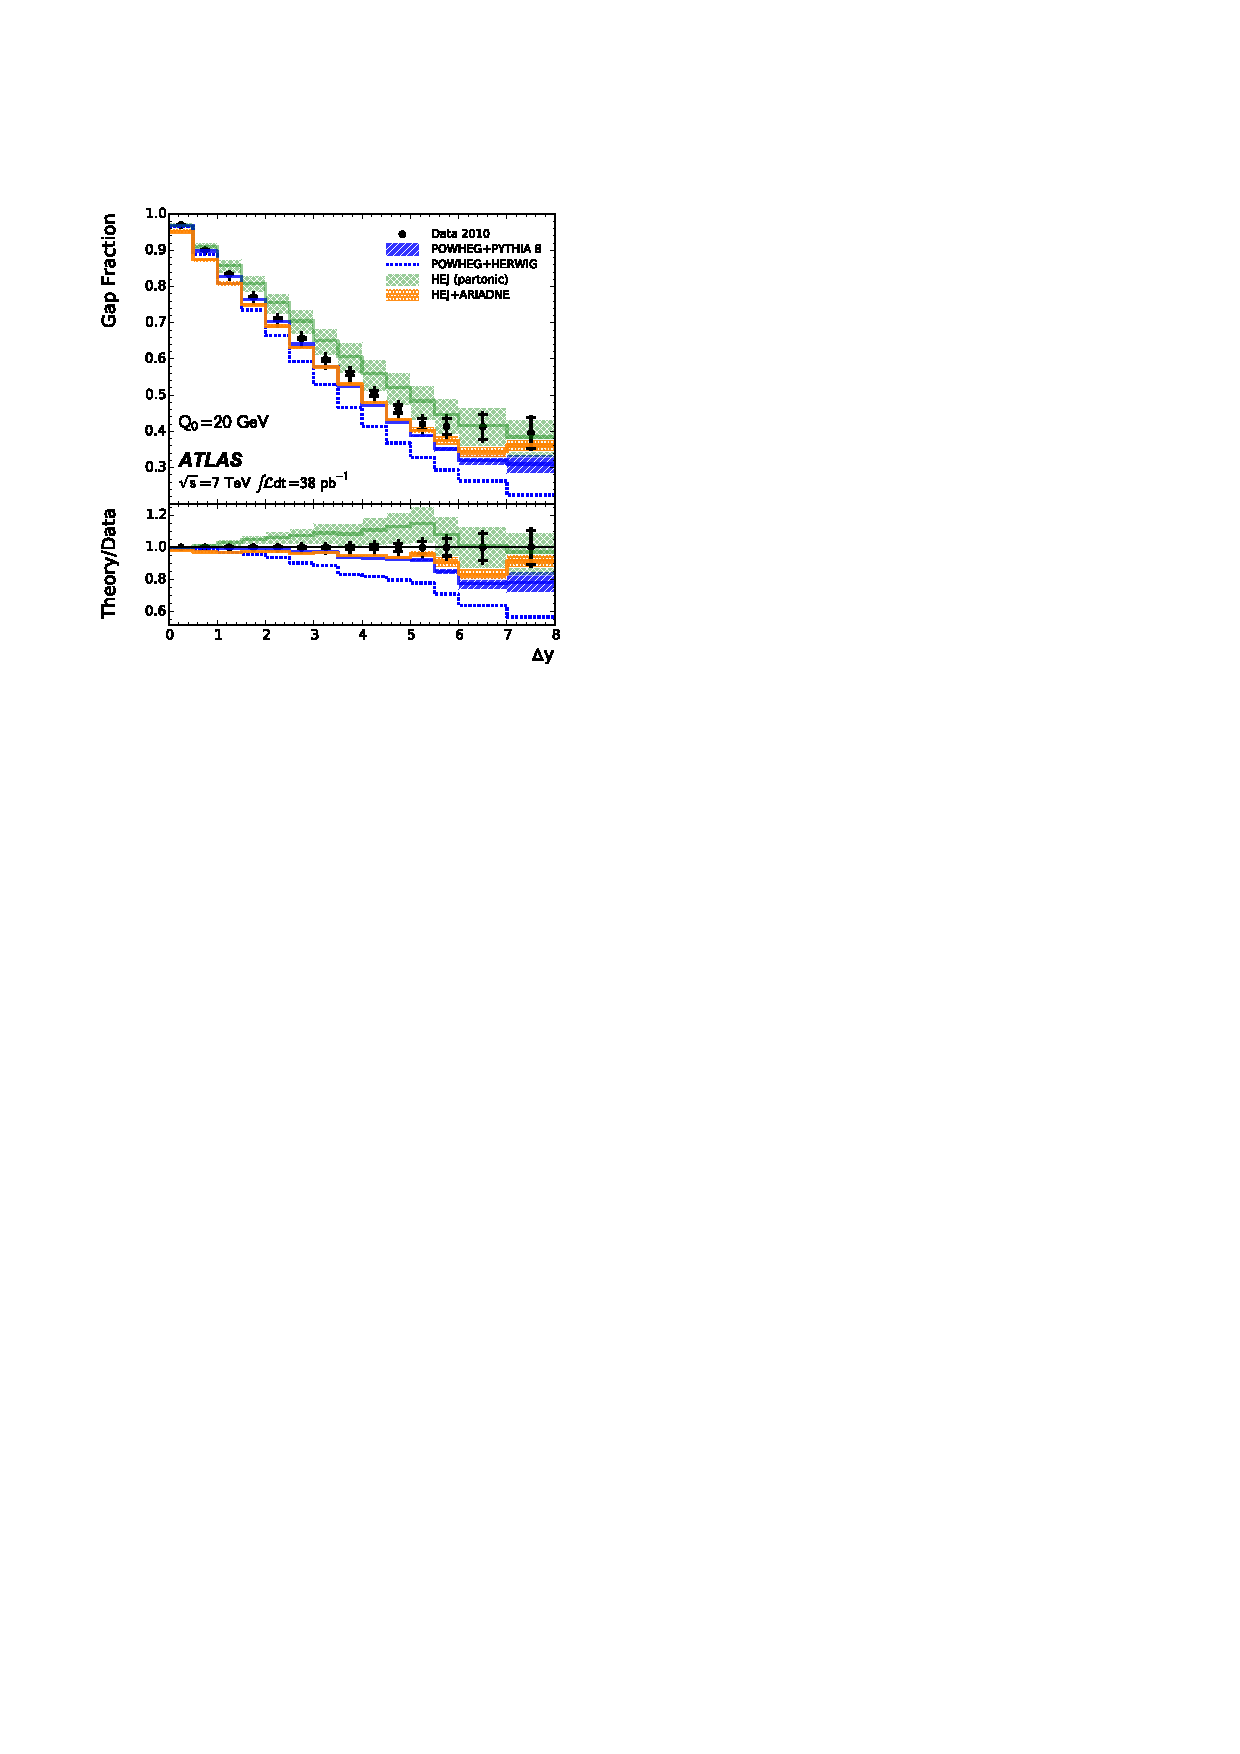
\includegraphics[width=\textwidth, height=1.0\textwidth]{pureJets3a}
			\caption{}
			\label{fig:}
		\end{subfigure}
		~
		\begin{subfigure}[b]{0.48\textwidth}
			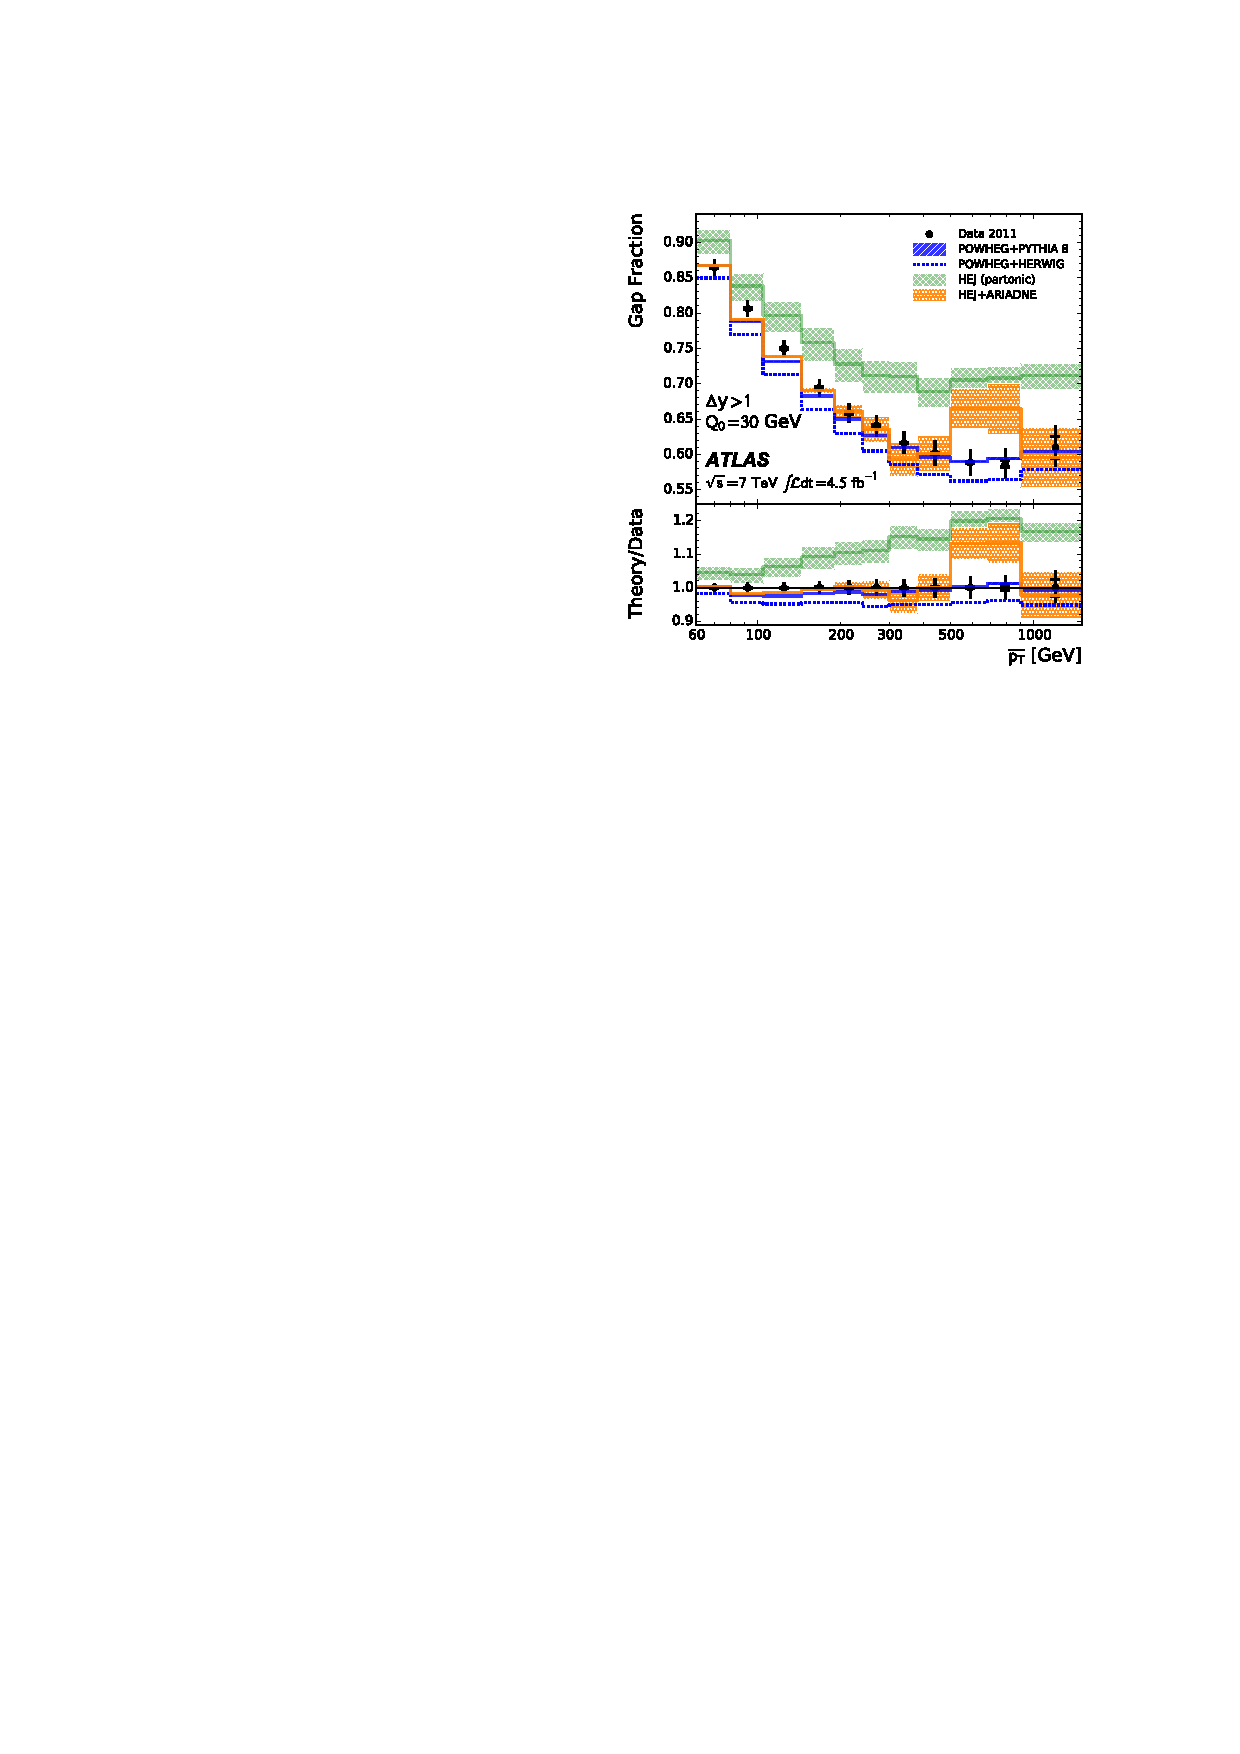
\includegraphics[width=\textwidth, height=1.0\textwidth]{pureJets3b}
			\caption{}
			\label{fig:}
		\end{subfigure}
		\caption{The gap fraction, $f(Q_0)$, as a function of (a) the rapidity gap, $\Delta y$, and (b) the average $p_T$, $\overline{p_T}$, of the dijet system.}
		\label{fig:}

		\begin{subfigure}[b]{0.48\textwidth}
			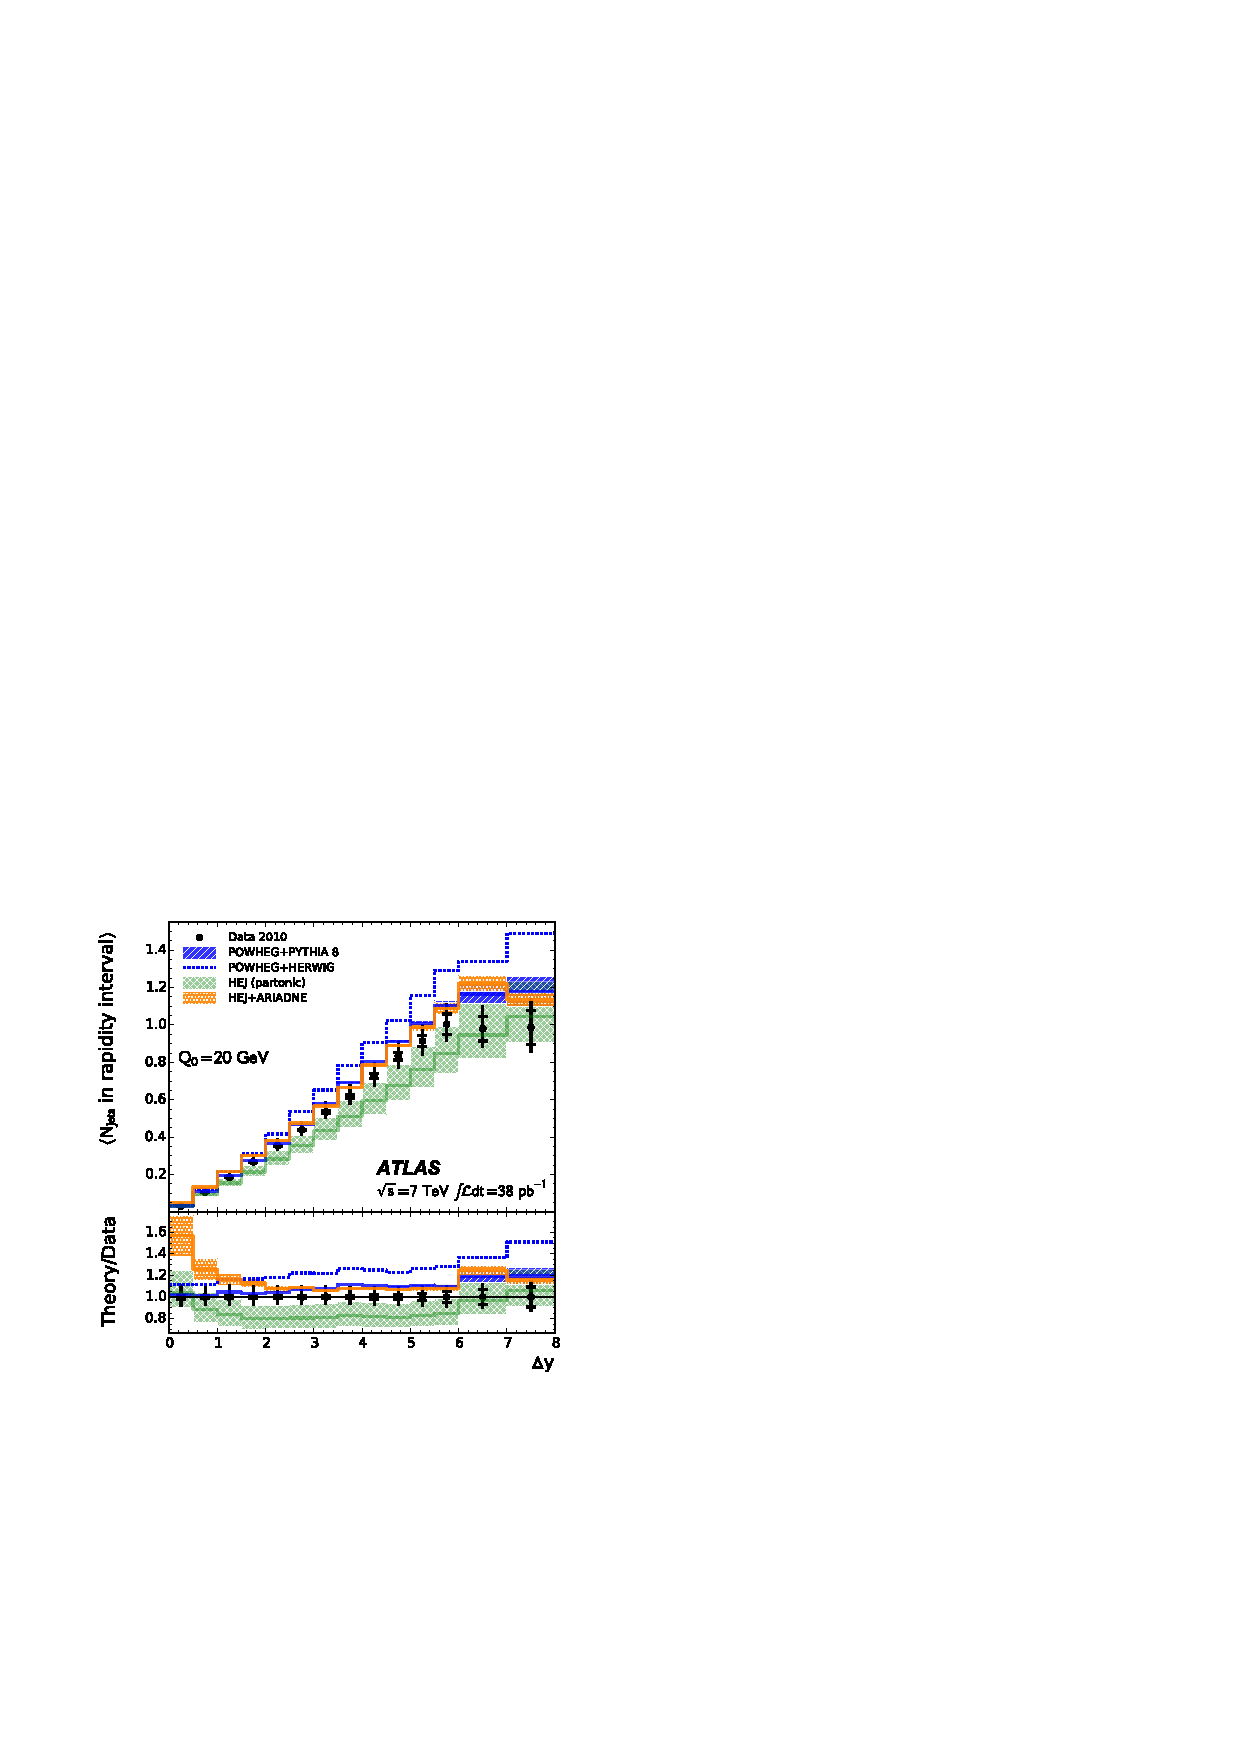
\includegraphics[width=\textwidth, height=1.0\textwidth]{pureJets4a}
			\caption{}
			\label{fig:}
		\end{subfigure}
		~
		\begin{subfigure}[b]{0.48\textwidth}
			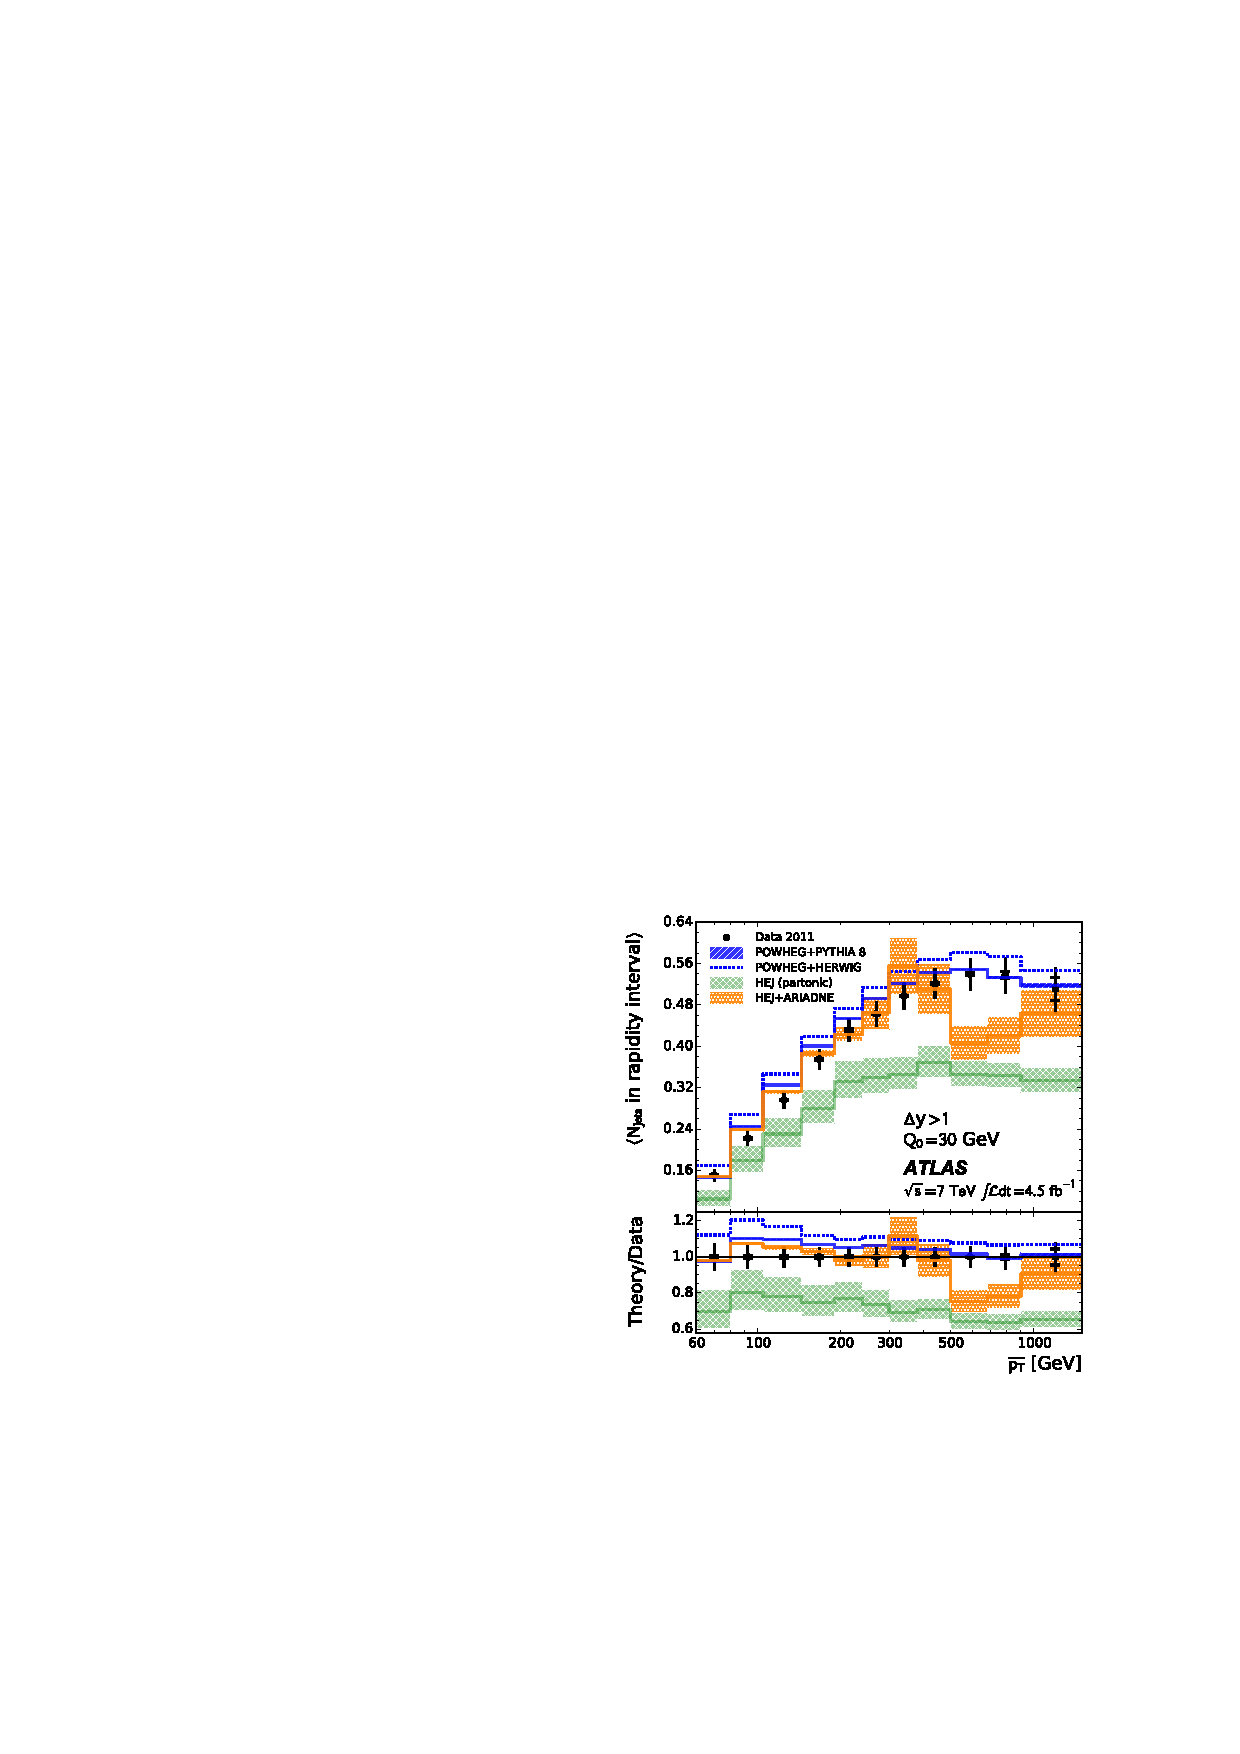
\includegraphics[width=\textwidth, height=1.0\textwidth]{pureJets4b}
			\caption{}
			\label{fig:}
		\end{subfigure}
		\caption{The average number of jets, $\langle N_{\text{jets}} \text{ in the rapidity interval}\rangle$, in the rapidity gap
		         bounded by the dijet system, as a function of (a) the rapidity gap, $\Delta y$, and (b) the average $p_T$, $\overline{p_T}$,
		         of the dijet system.}
		\label{fig:}
	\end{figure}

	\begin{figure}[H]
		\centering
		\begin{subfigure}[b]{0.48\textwidth}
			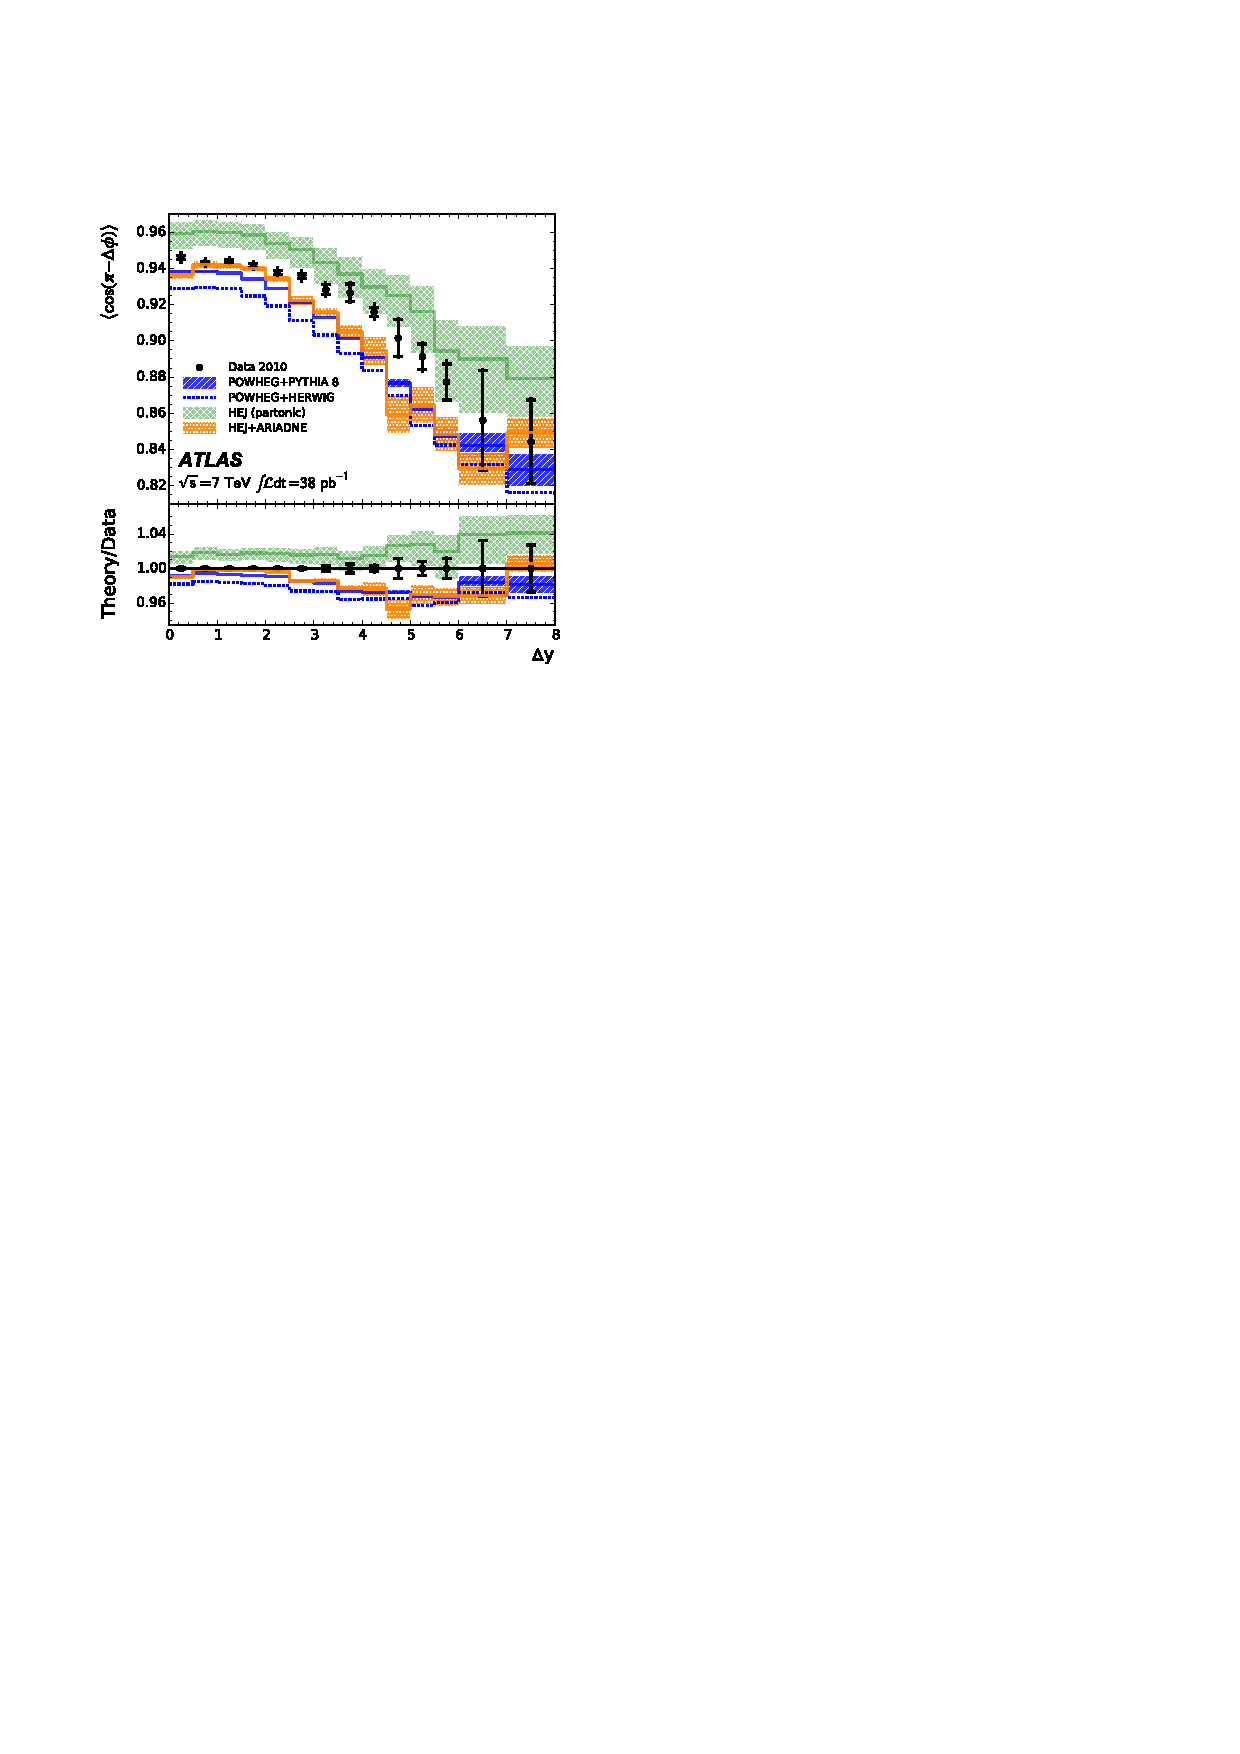
\includegraphics[width=\textwidth, height=1.0\textwidth]{pureJets5a}
			\caption{}
			\label{fig:}
		\end{subfigure}
		~
		\begin{subfigure}[b]{0.48\textwidth}
			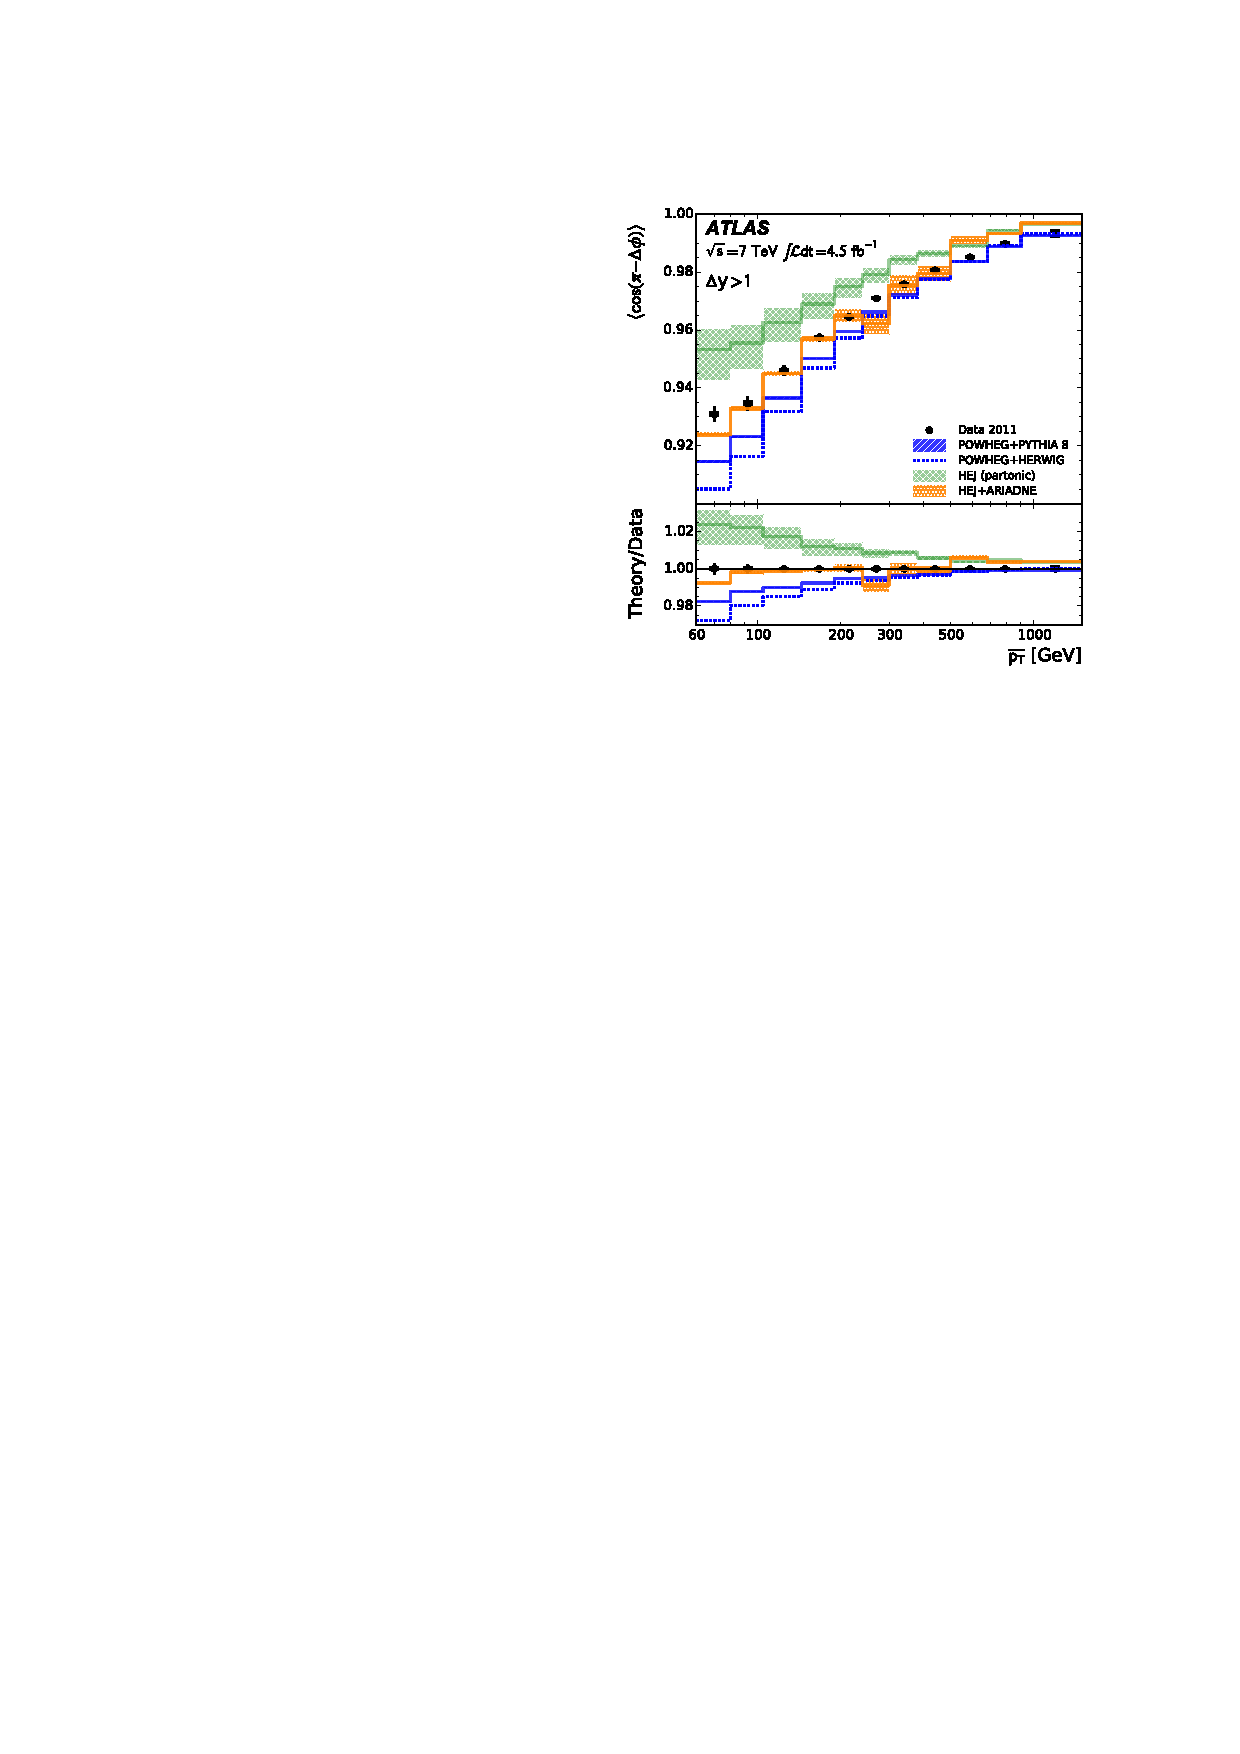
\includegraphics[width=\textwidth, height=1.0\textwidth]{pureJets5b}
			\caption{}
			\label{fig:}
		\end{subfigure}
		\caption{The first azimuthal anglular moment, $\langle \cos(\pi-\Delta\phi)\rangle$, as a function of (a) the rapidity gap, $\Delta y$
		         and (b) the average $p_T$, $\overline{p_T}$, of the dijet system.}
		\label{fig:}

		\begin{subfigure}[b]{0.48\textwidth}
			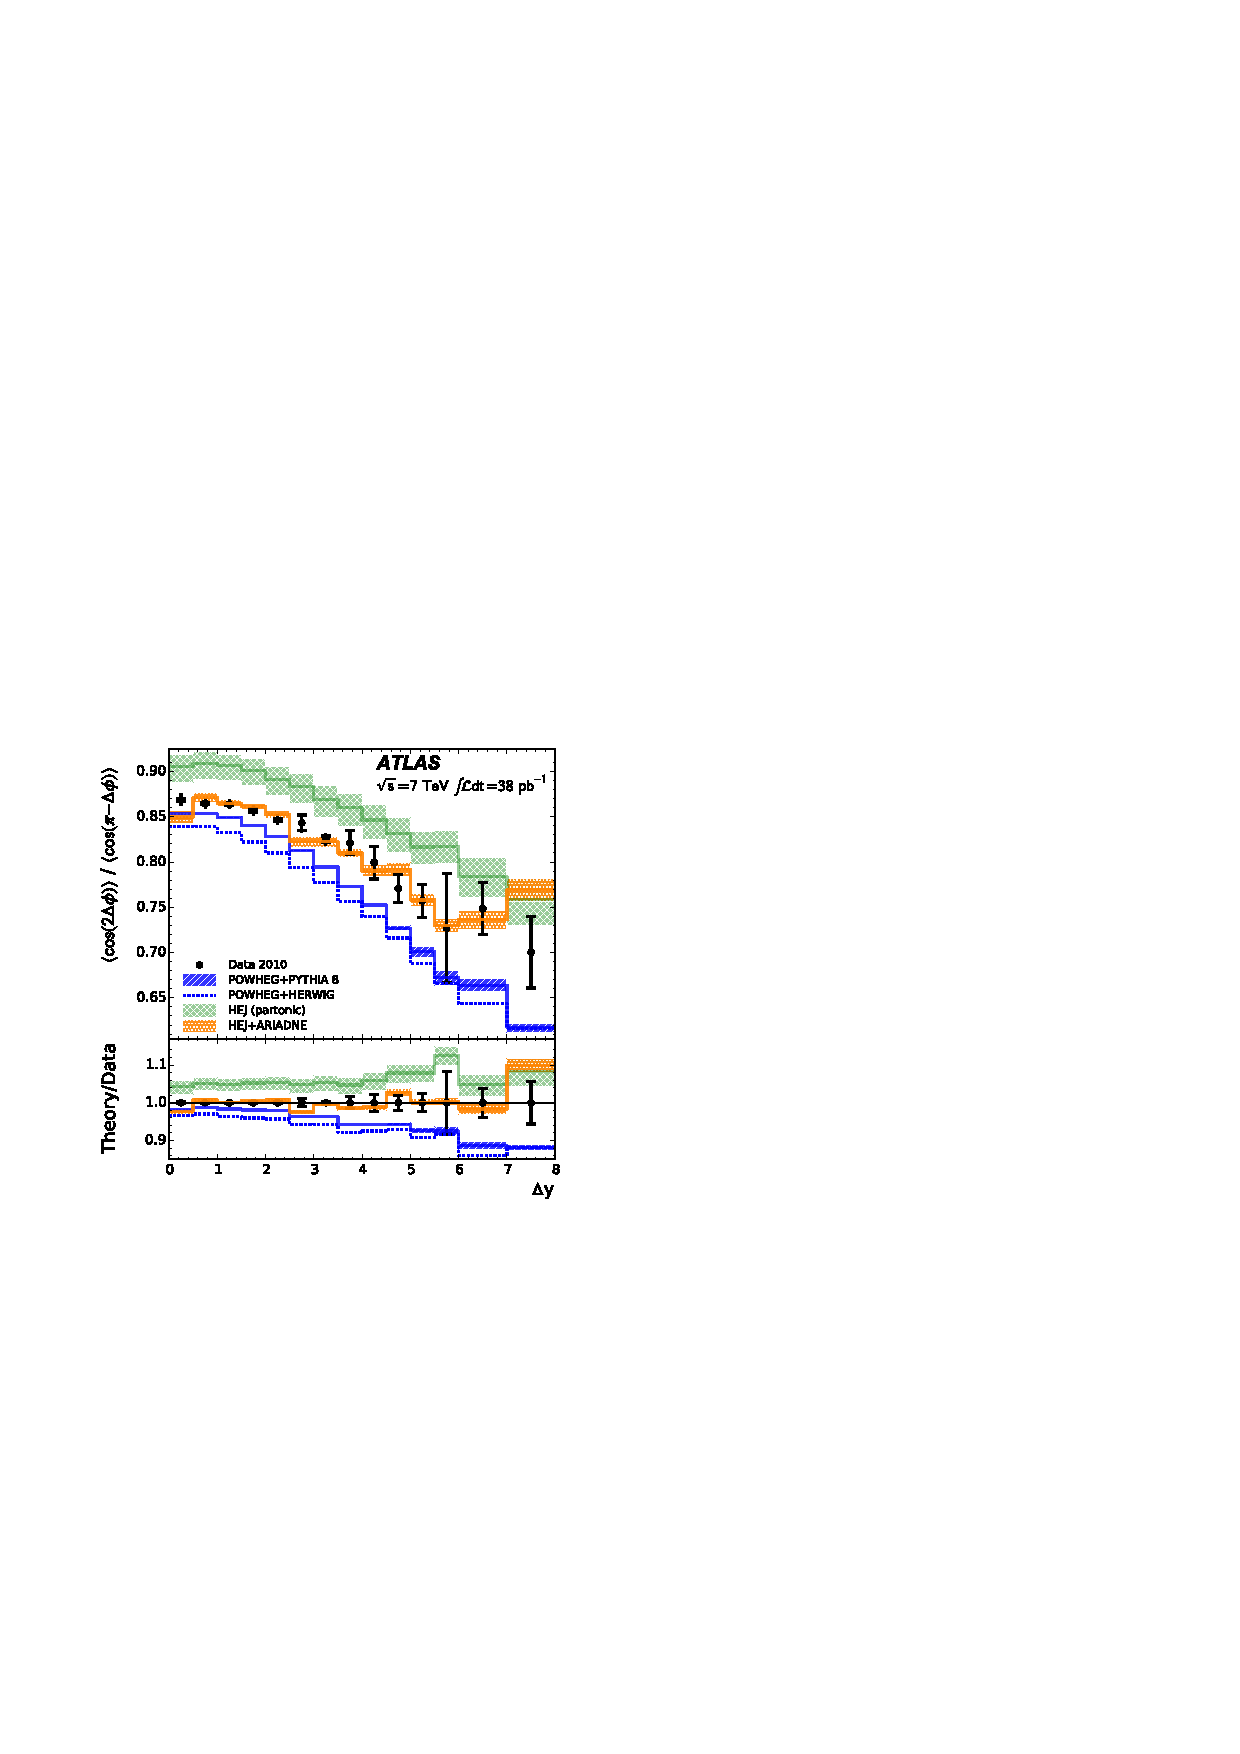
\includegraphics[width=\textwidth, height=1.0\textwidth]{pureJets5c}
			\caption{}
			\label{fig:}
		\end{subfigure}
		~
		\begin{subfigure}[b]{0.48\textwidth}
			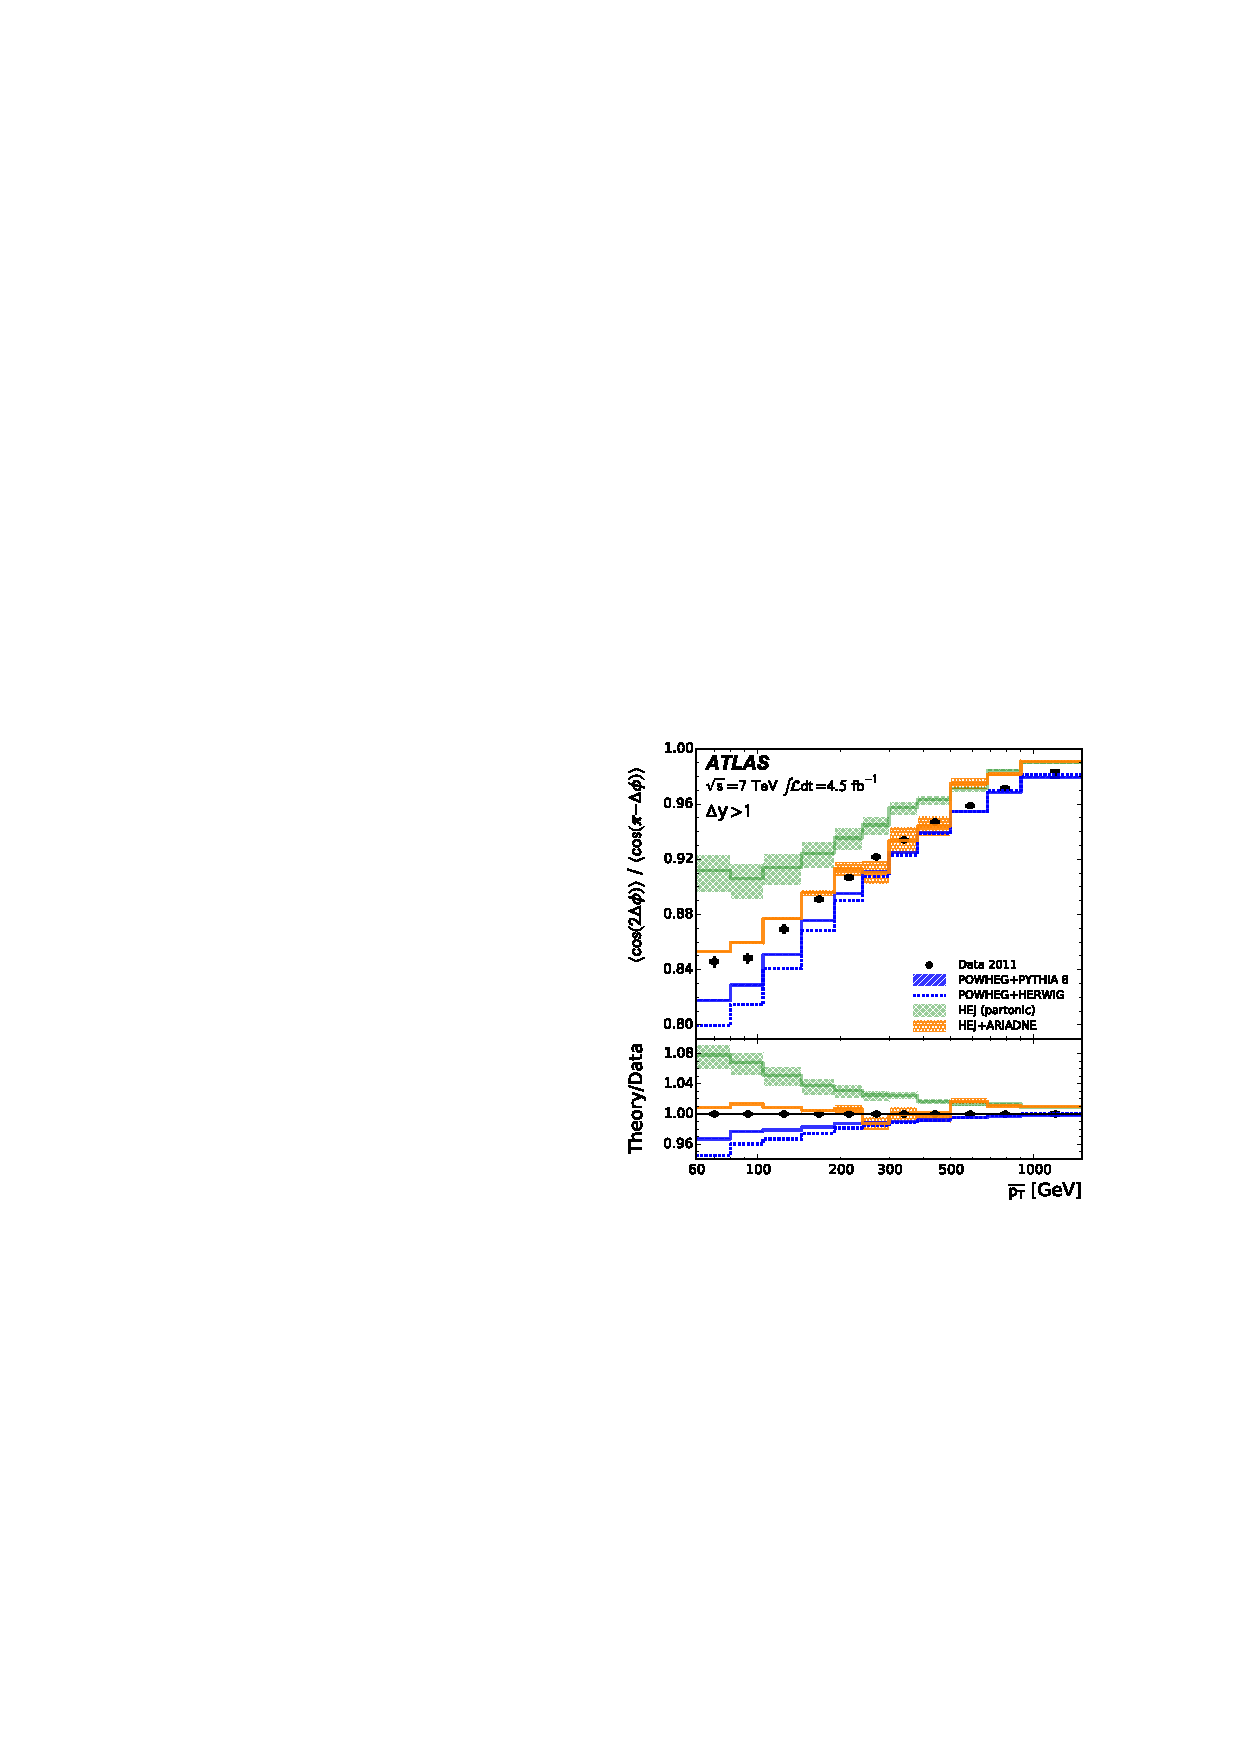
\includegraphics[width=\textwidth, height=1.0\textwidth]{pureJets5d}
			\caption{}
			\label{fig:}
		\end{subfigure}
		\caption{The ratio of the second azimuthal anglular moment, $\langle \cos(2\Delta\phi)\rangle$, to the first azimuthal
		         anglular moment, $\langle \cos(\pi-\Delta\phi)\rangle$, as a function of (a) the rapidity gap, $\Delta y$, and (b) the
		         average $p_T$, $\overline{p_T}$, of the dijet system.}
		\label{fig:}
	\end{figure}

	\begin{figure}[H]
		\centering
		\begin{subfigure}[b]{0.48\textwidth}
			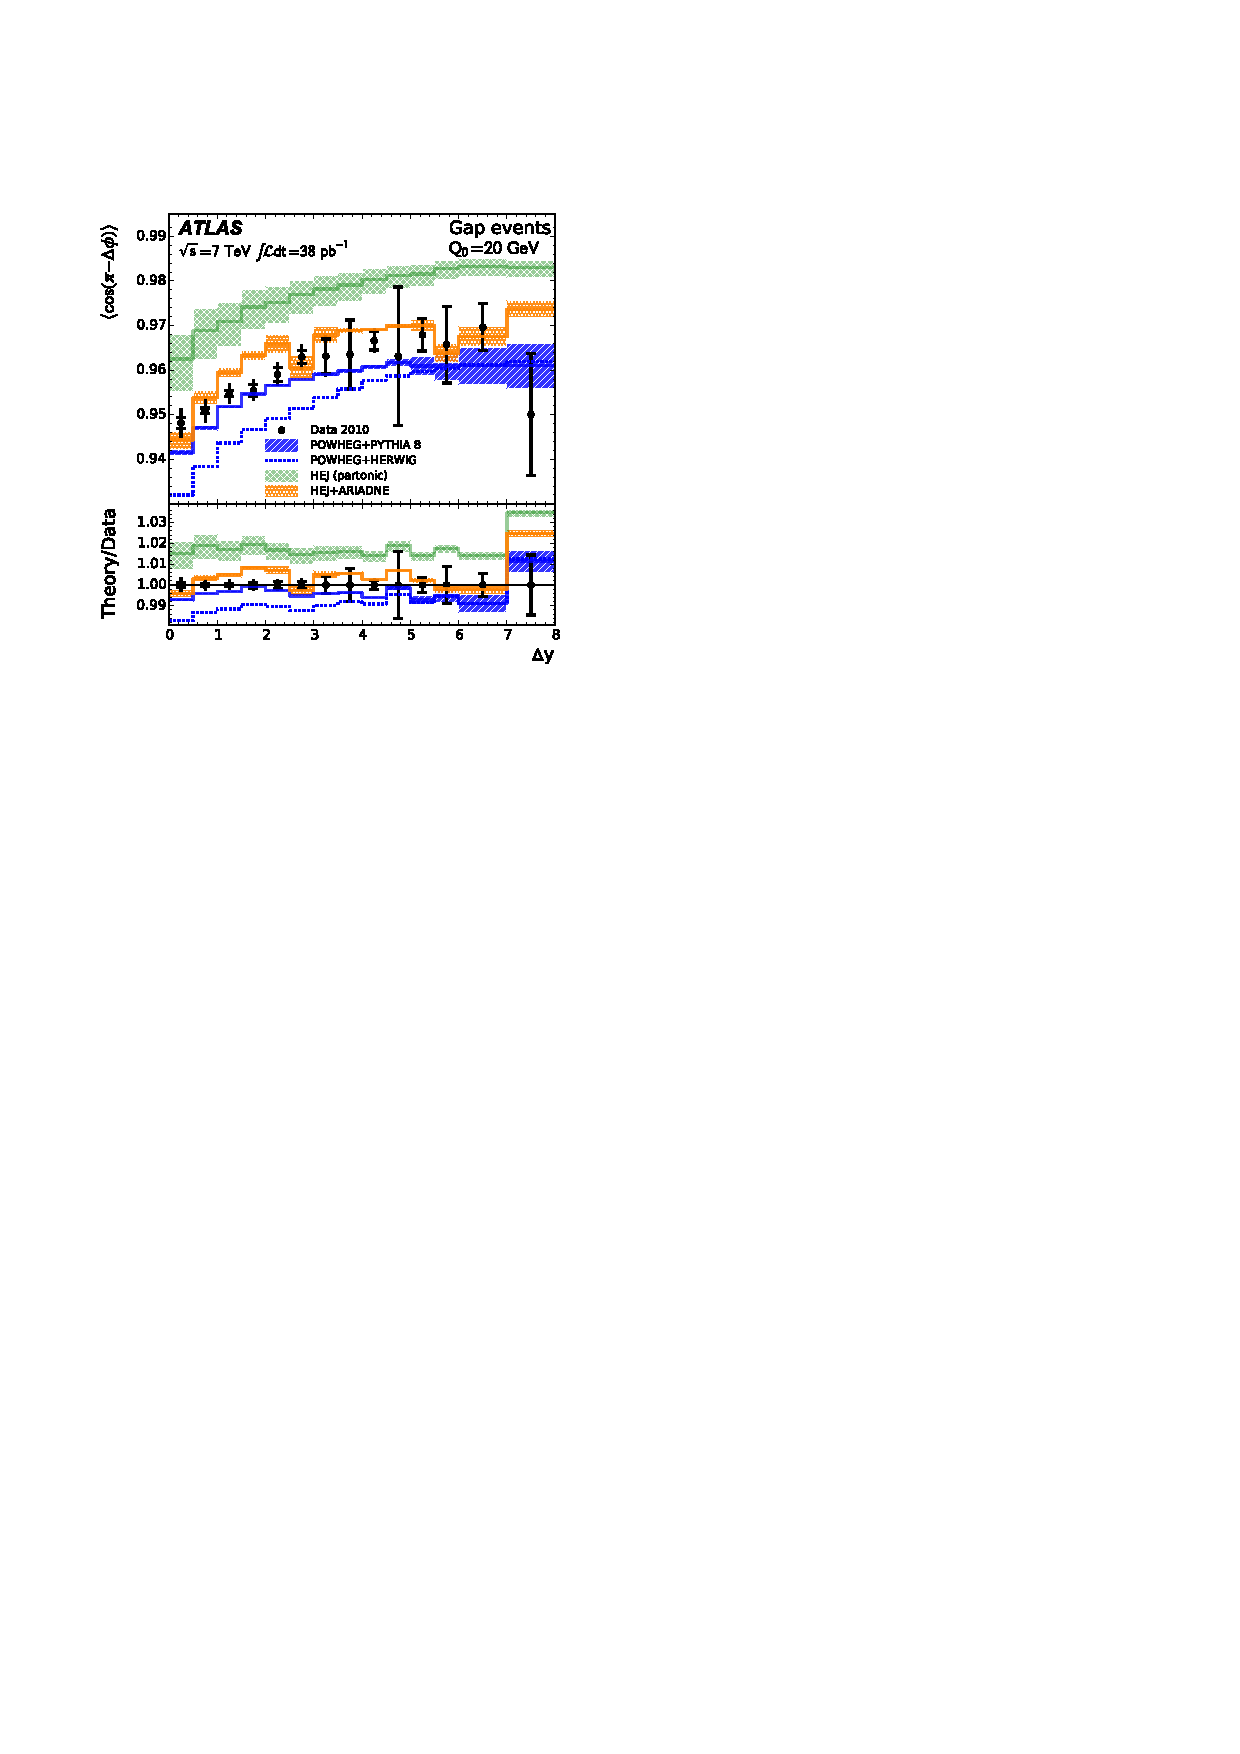
\includegraphics[width=\textwidth, height=1.0\textwidth]{pureJets6a}
			\caption{}
			\label{fig:}
		\end{subfigure}
		~
		\begin{subfigure}[b]{0.48\textwidth}
			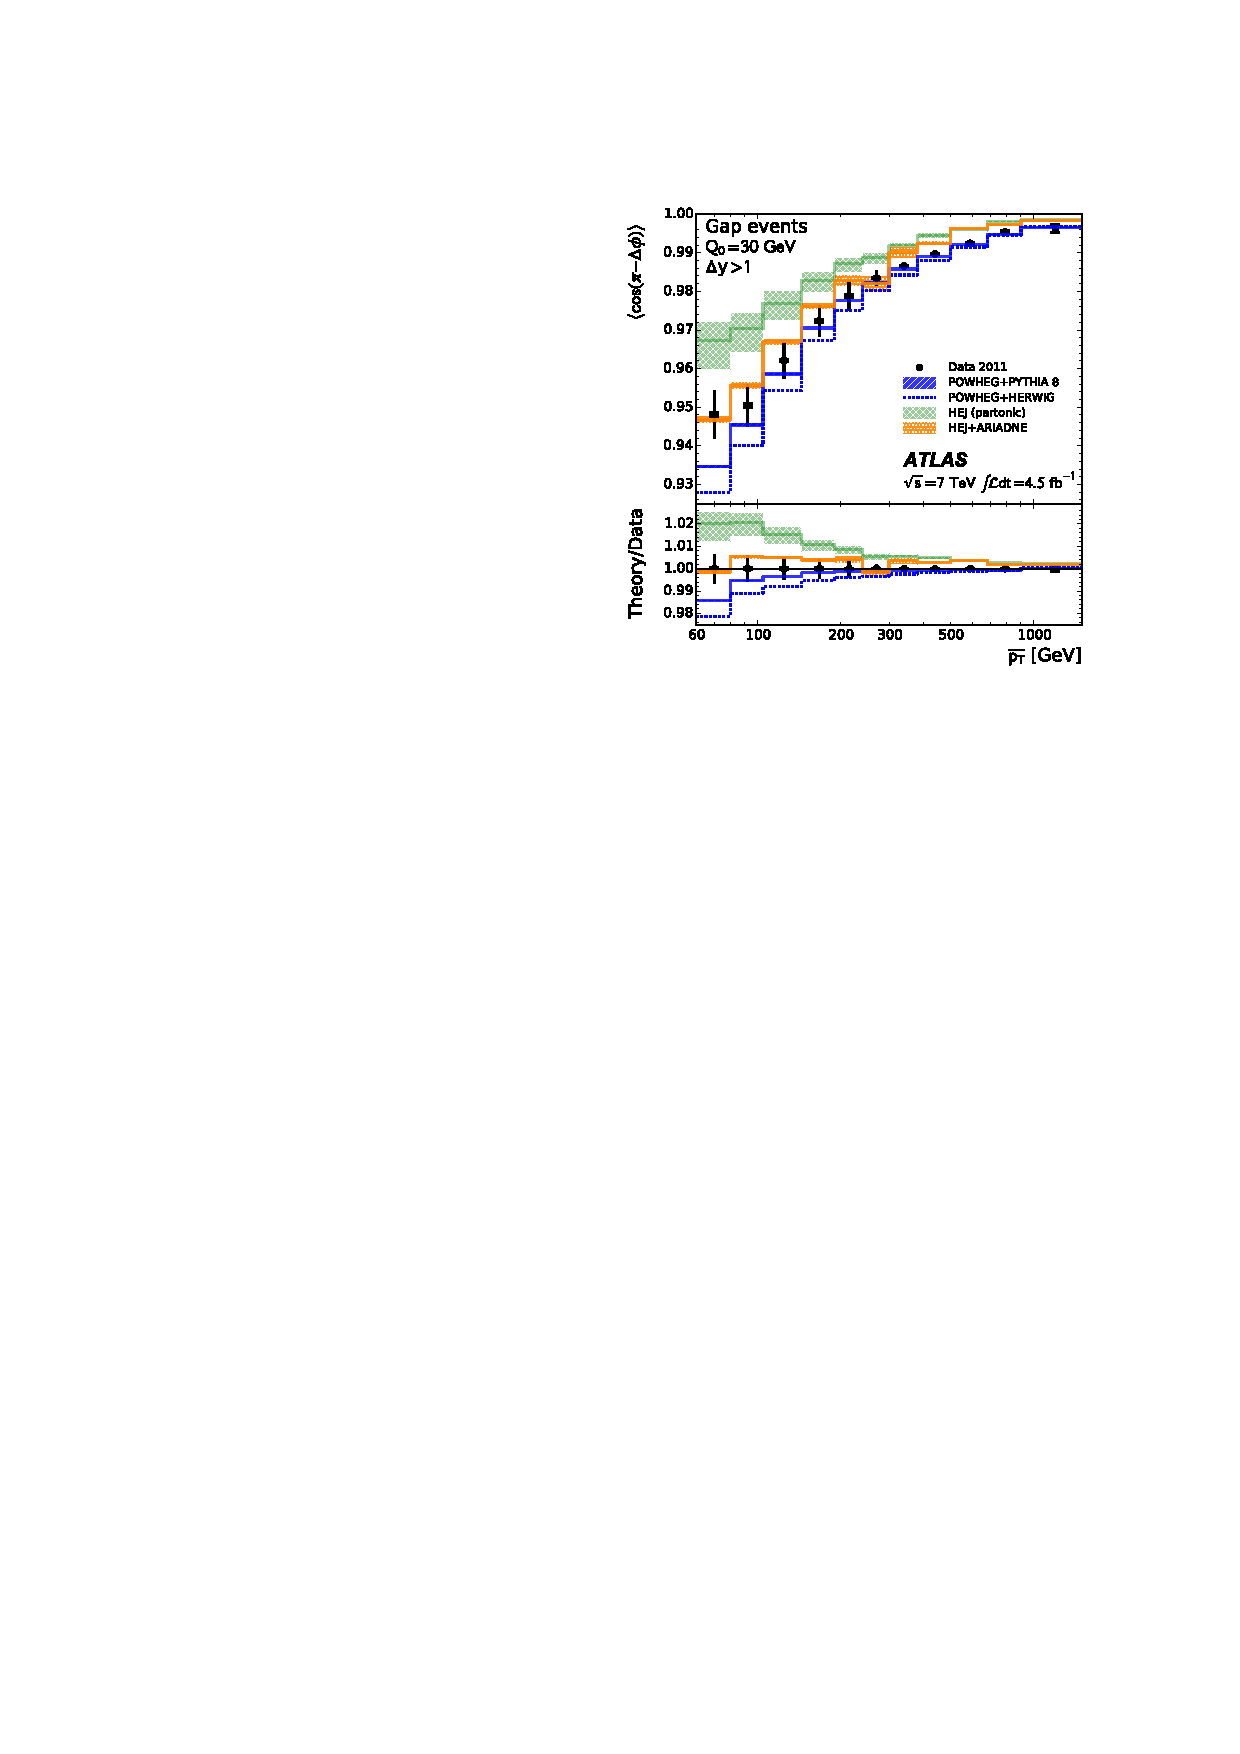
\includegraphics[width=\textwidth, height=1.0\textwidth]{pureJets6b}
			\caption{}
			\label{fig:}
		\end{subfigure}
		\caption{The first azimuthal anglular moment, $\langle \cos(\pi-\Delta\phi)\rangle$, for events passing the veto on gap activity
		         above $Q_0=20\text{GeV}$ as a function of (a) the rapidity gap, $\Delta y$, and (b) the average $p_T$, $\overline{p_T}$,
		         of the dijet system.}
		\label{fig:}

		\begin{subfigure}[b]{0.48\textwidth}
			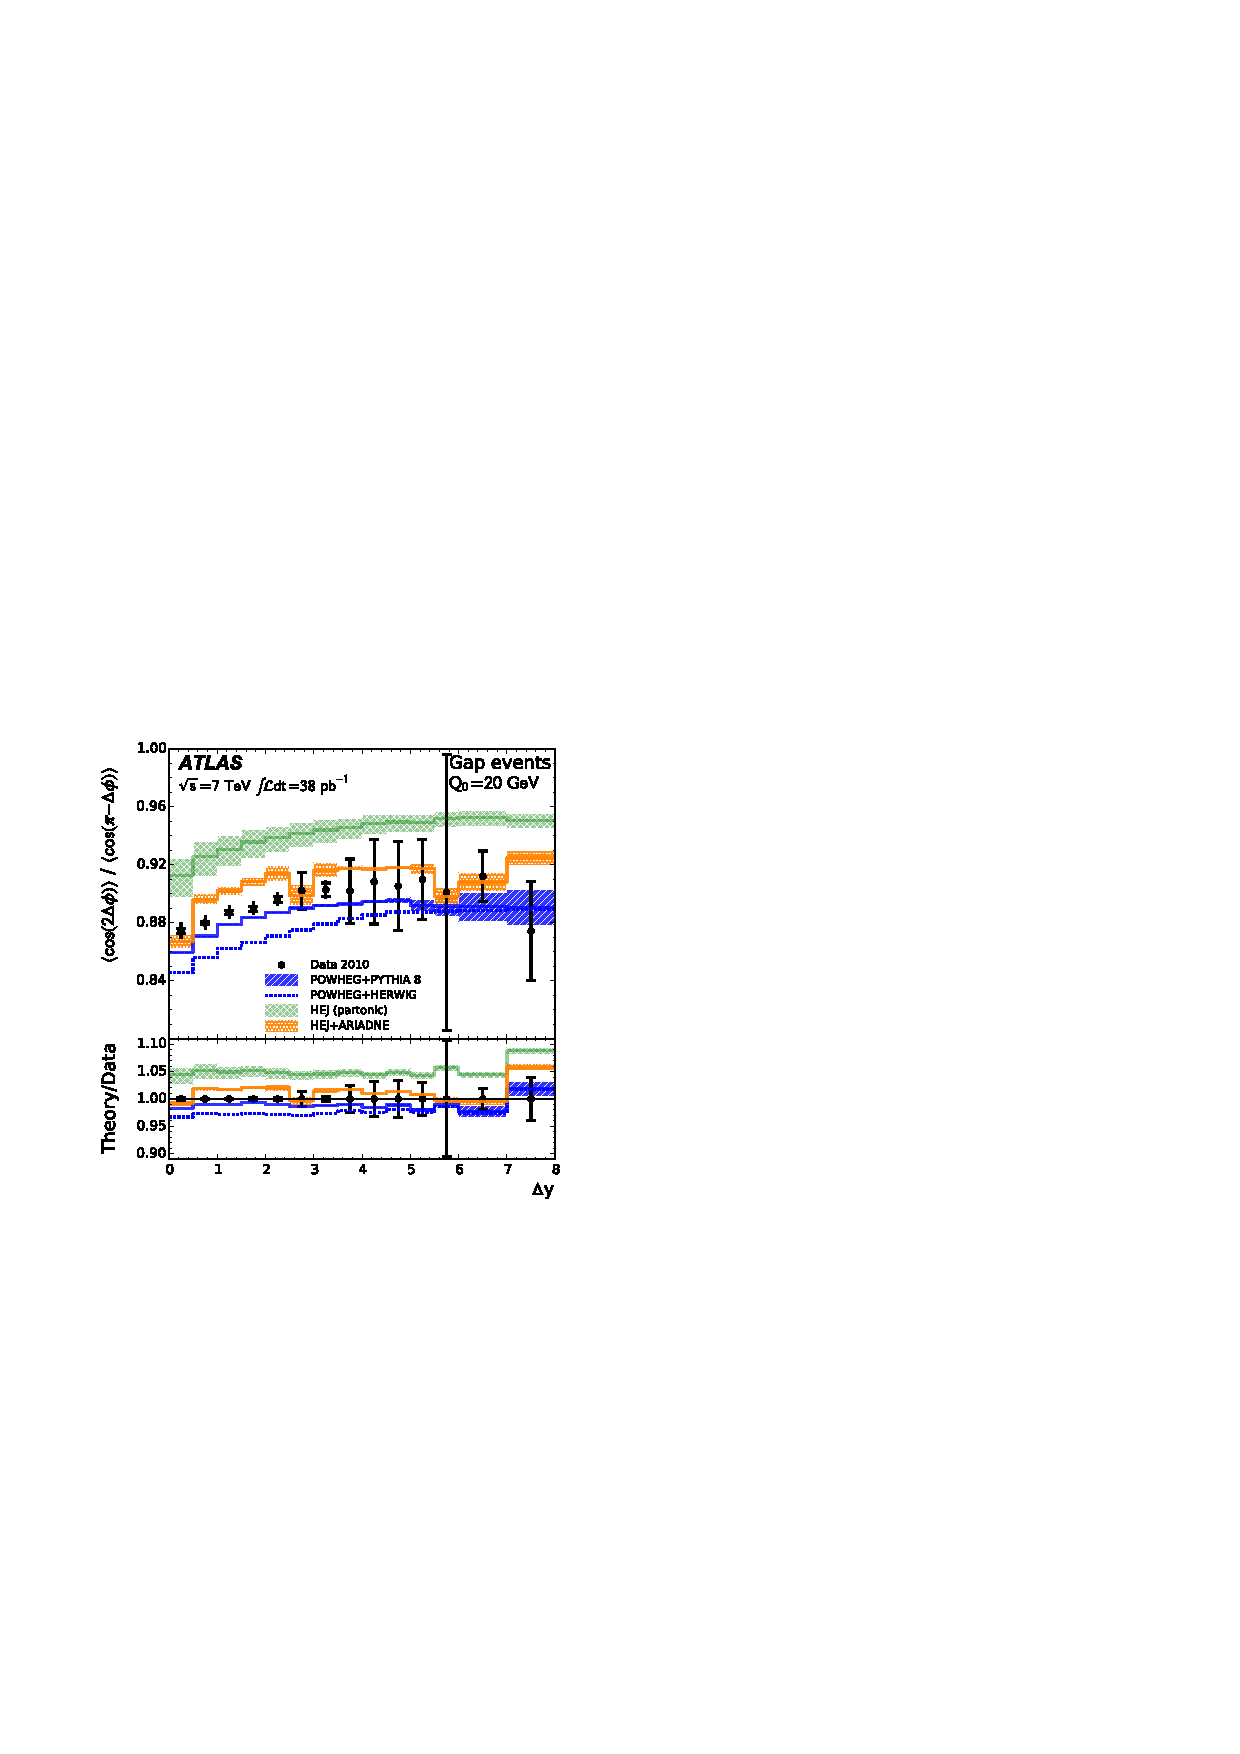
\includegraphics[width=\textwidth, height=1.0\textwidth]{pureJets6c}
			\caption{}
			\label{fig:}
		\end{subfigure}
		~
		\begin{subfigure}[b]{0.48\textwidth}
			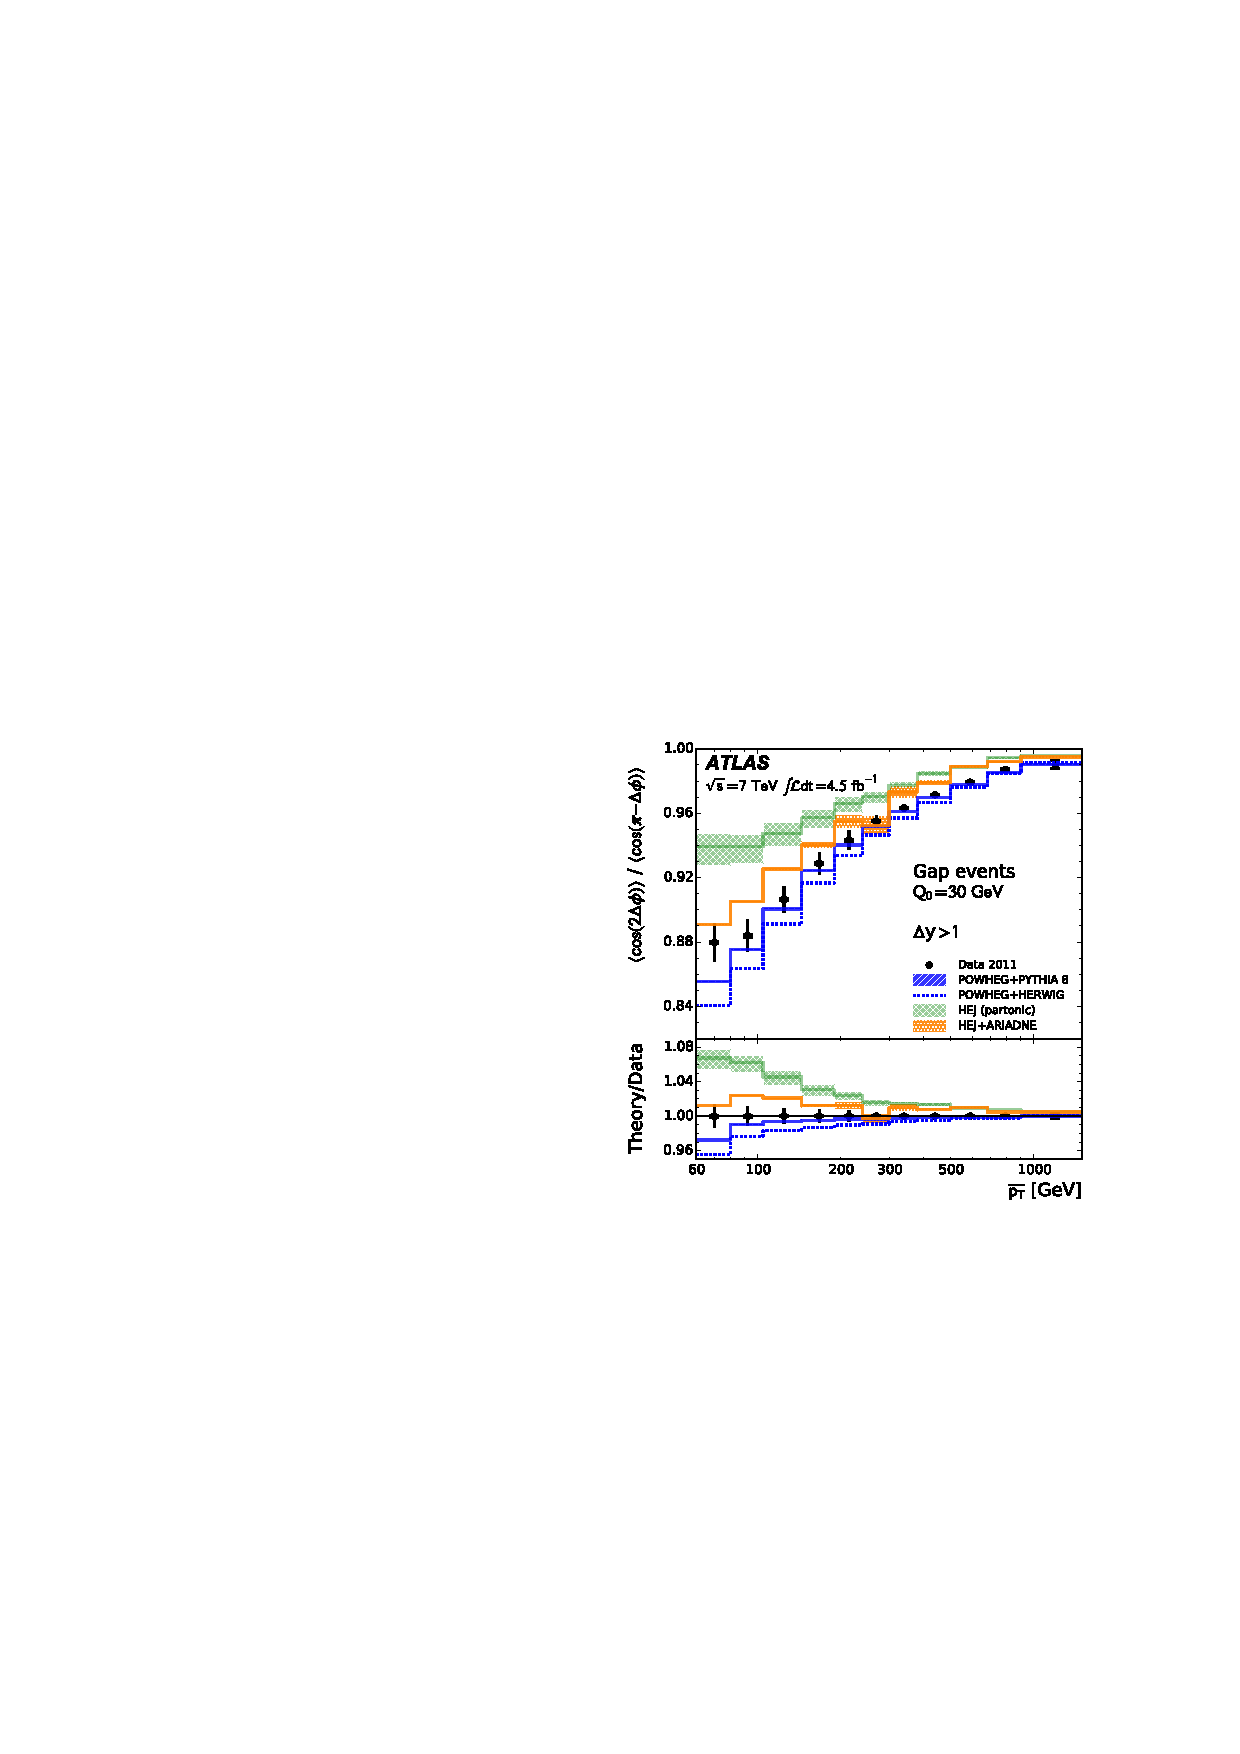
\includegraphics[width=\textwidth, height=1.0\textwidth]{pureJets6d}
			\caption{}
			\label{fig:}
		\end{subfigure}
		\caption{The ratio of the second azimuthal anglular moment, $\langle \cos(2\Delta\phi)\rangle$, to the first azimuthal
		         anglular moment, $\langle \cos(\pi-\Delta\phi)\rangle$, as a function of (a) the rapidity gap, $\Delta y$, and (b) the
		         average $p_T$, $\overline{p_T}$, of the dijet system.  A veto of $Q_0=20\text{GeV}$, for (a), and $Q_0=30\text{GeV}$,
		         for (b), is applied on activity in the rapidity gap is applied.}
		\label{fig:}
	\end{figure}

	\begin{figure}[H]
		\centering
		\begin{subfigure}[b]{0.48\textwidth}
			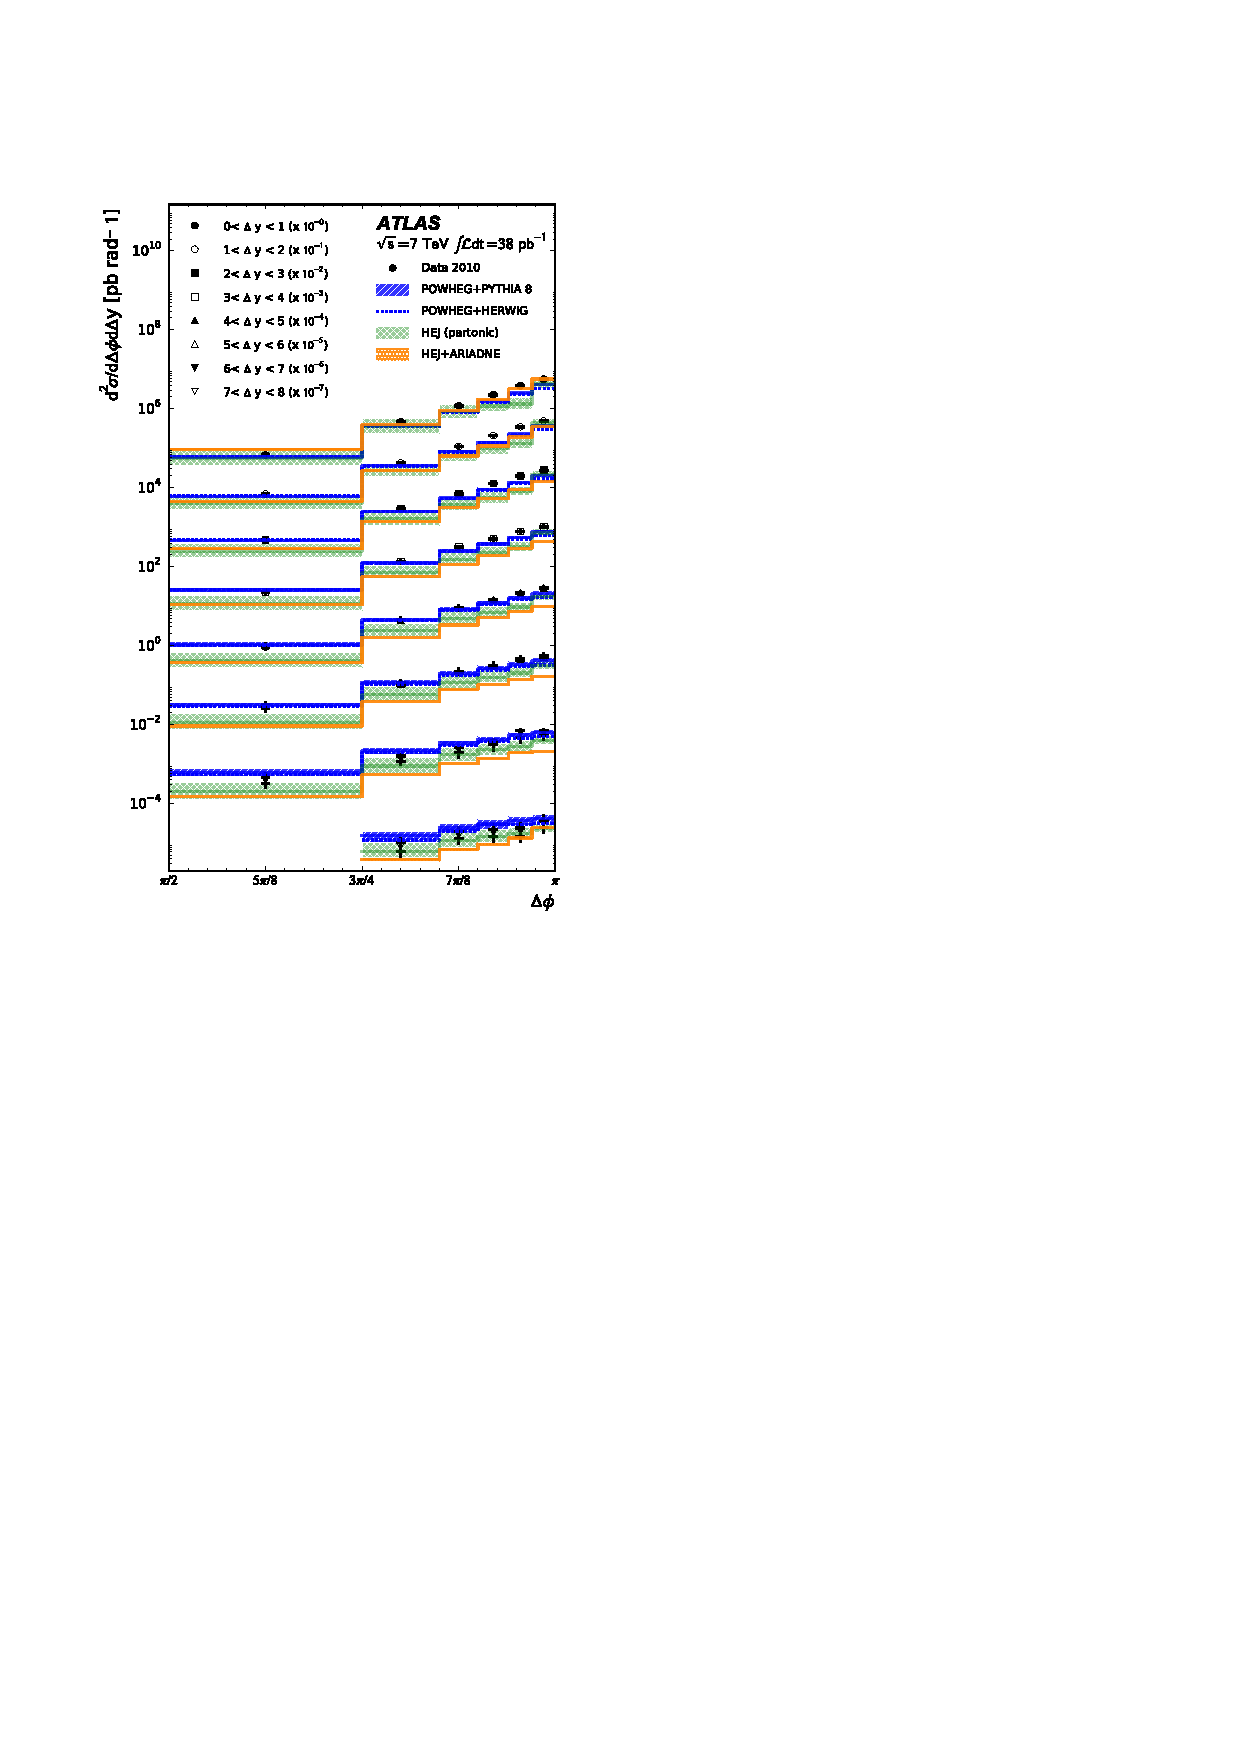
\includegraphics[width=\textwidth, height=1.1\textwidth]{pureJets7a}
			\caption{}
			\label{fig:}
		\end{subfigure}
		~
		\begin{subfigure}[b]{0.48\textwidth}
			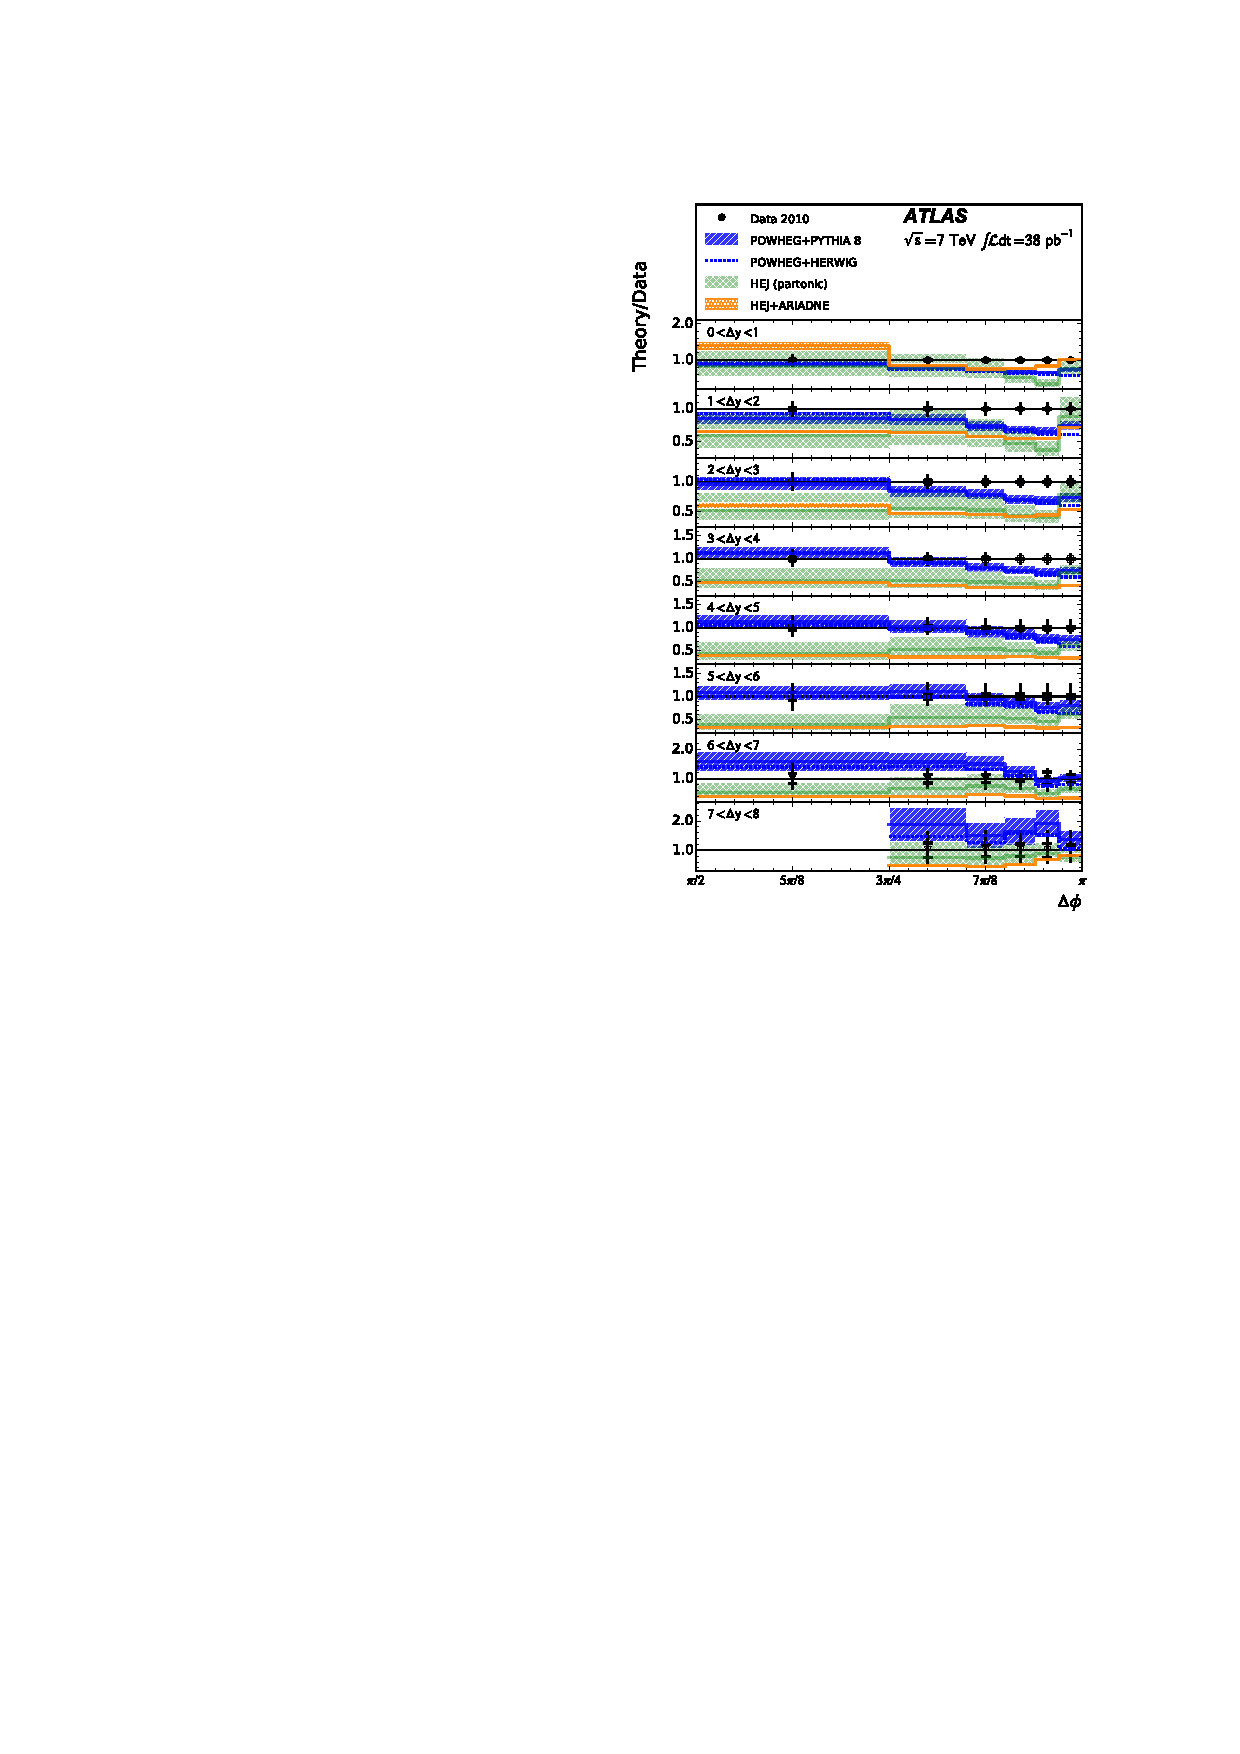
\includegraphics[width=\textwidth, height=1.1\textwidth]{pureJets7b}
			\caption{}
			\label{fig:}
		\end{subfigure}
		\caption{The double-differential cross-section as a function of the azimuthal seperation, $\Delta\phi$,
		         and the rapidity gap, $\Delta y$, of the dijet system.}
		\label{fig:}

		\begin{subfigure}[b]{0.48\textwidth}
			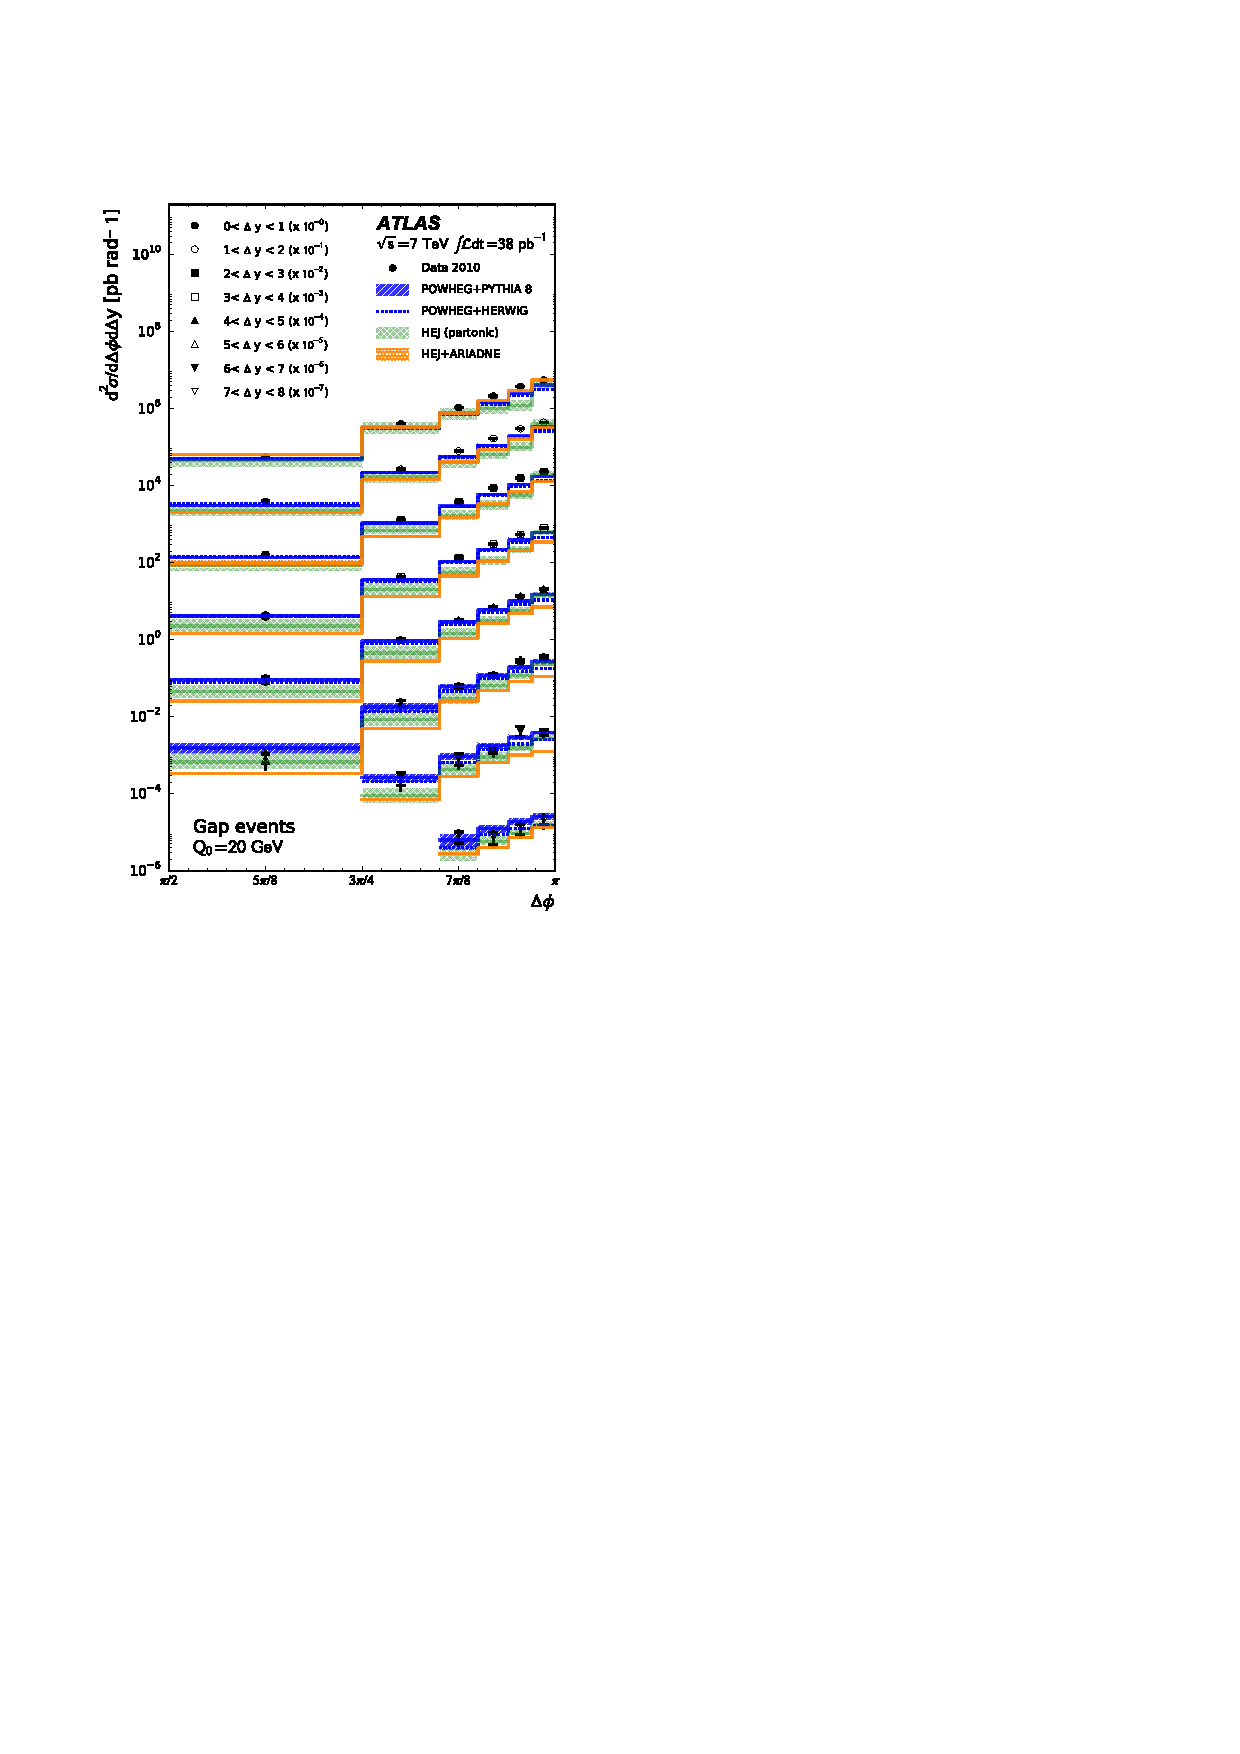
\includegraphics[width=\textwidth, height=1.1\textwidth]{pureJets8a}
			\caption{}
			\label{fig:}
		\end{subfigure}
		~
		\begin{subfigure}[b]{0.48\textwidth}
			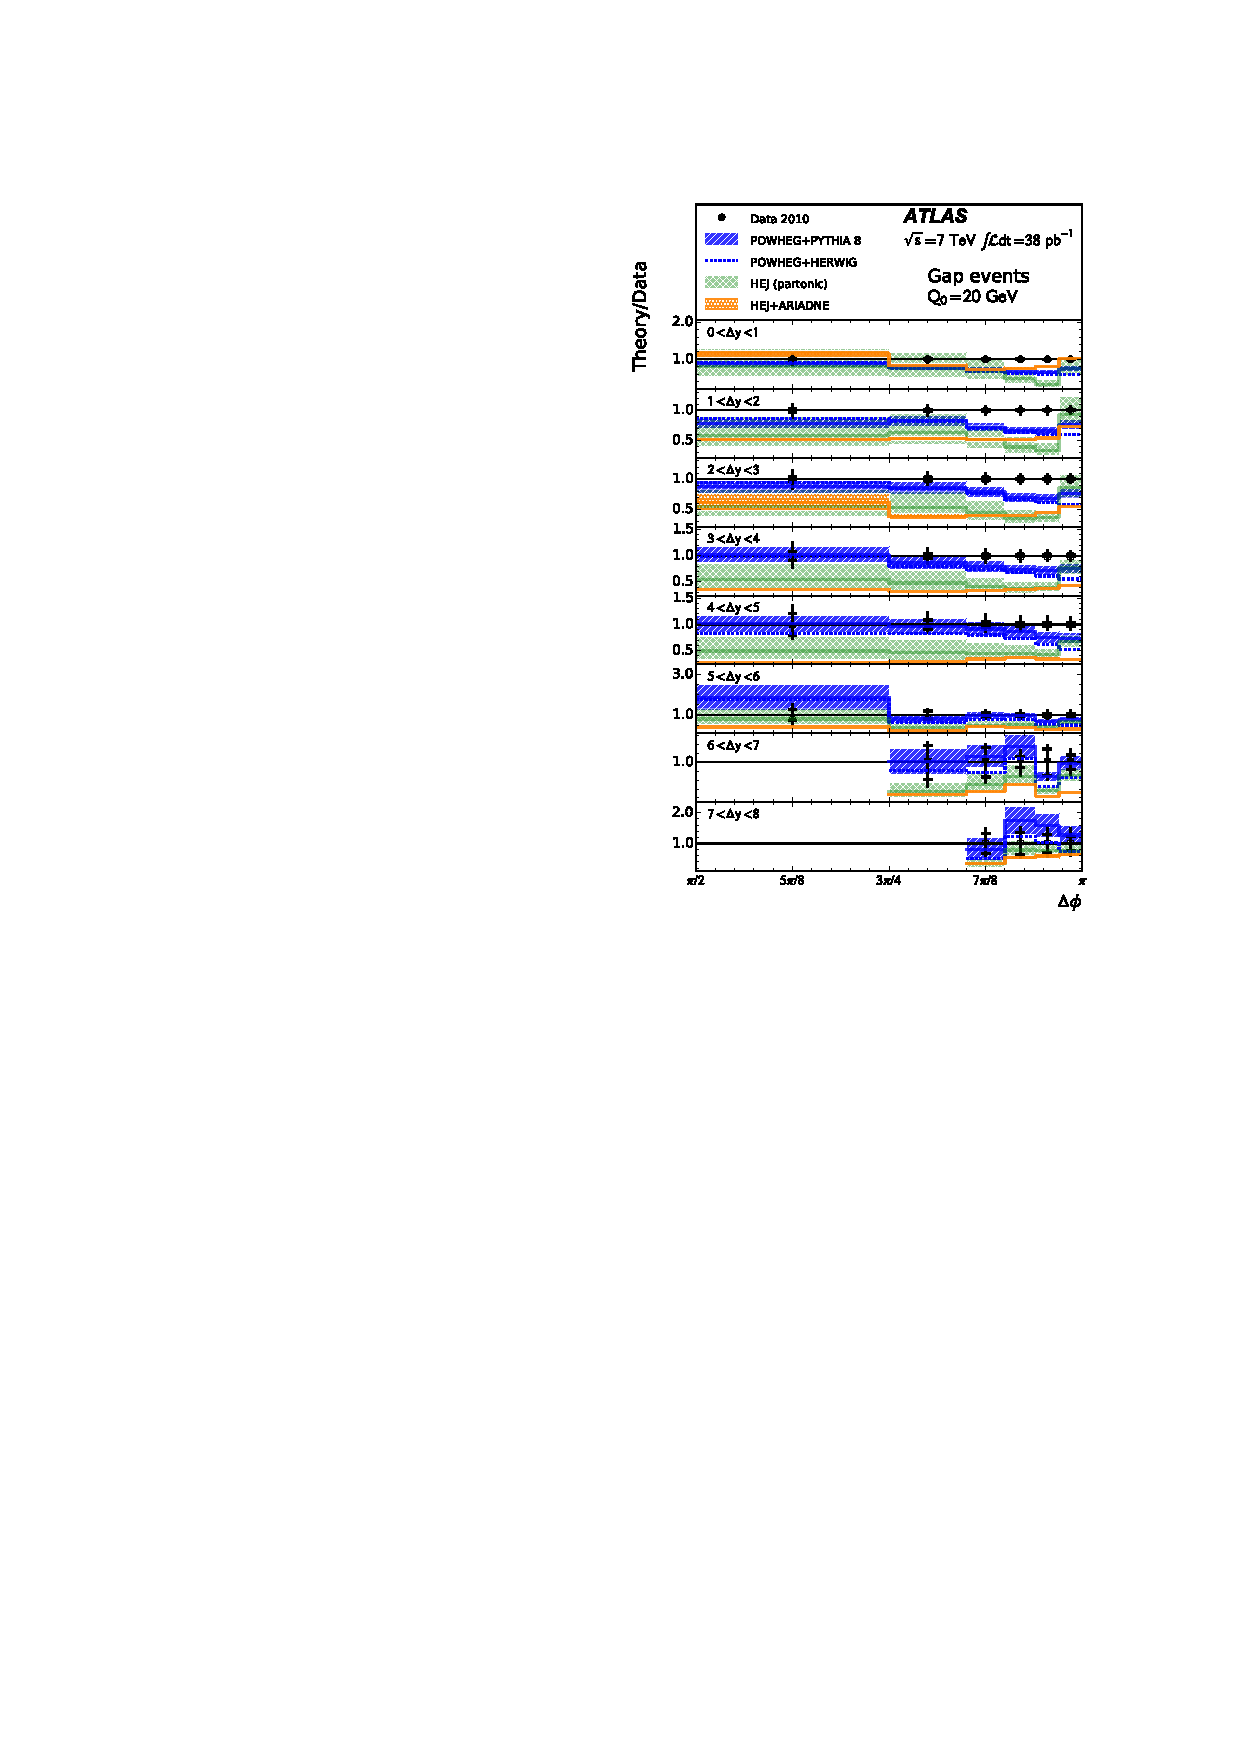
\includegraphics[width=\textwidth, height=1.1\textwidth]{pureJets8b}
			\caption{}
			\label{fig:}
		\end{subfigure}
		\caption{The double-differential cross-section as a function of the azimuthal seperation, $\Delta\phi$,
		         and the rapidity gap, $\Delta y$, of the dijet system.  A veto of $Q_0=20\text{GeV}$ is applied
		         on activity in the rapidity gap is applied.}
		\label{fig:}
	\end{figure}

\chapter{$\zg$+Jets at 100TeV}
\label{chap:100TeV}

	\begin{itemize}
		\item Talk about the FCC movement and the effect we expect the resummation will have at these energies.
		\item Put all three lines (30GeV, 60GeV, 100GeV) on the same plots in this section?
		\item Pros: Can see that we can put more stringent cuts while maintaining x-section.  Also
		      makes the point that we can cut out all the NP physics we cant model.
		\item Cons: Plots will be very busy.
	\end{itemize}

	\begin{figure}[h]
		\centering
		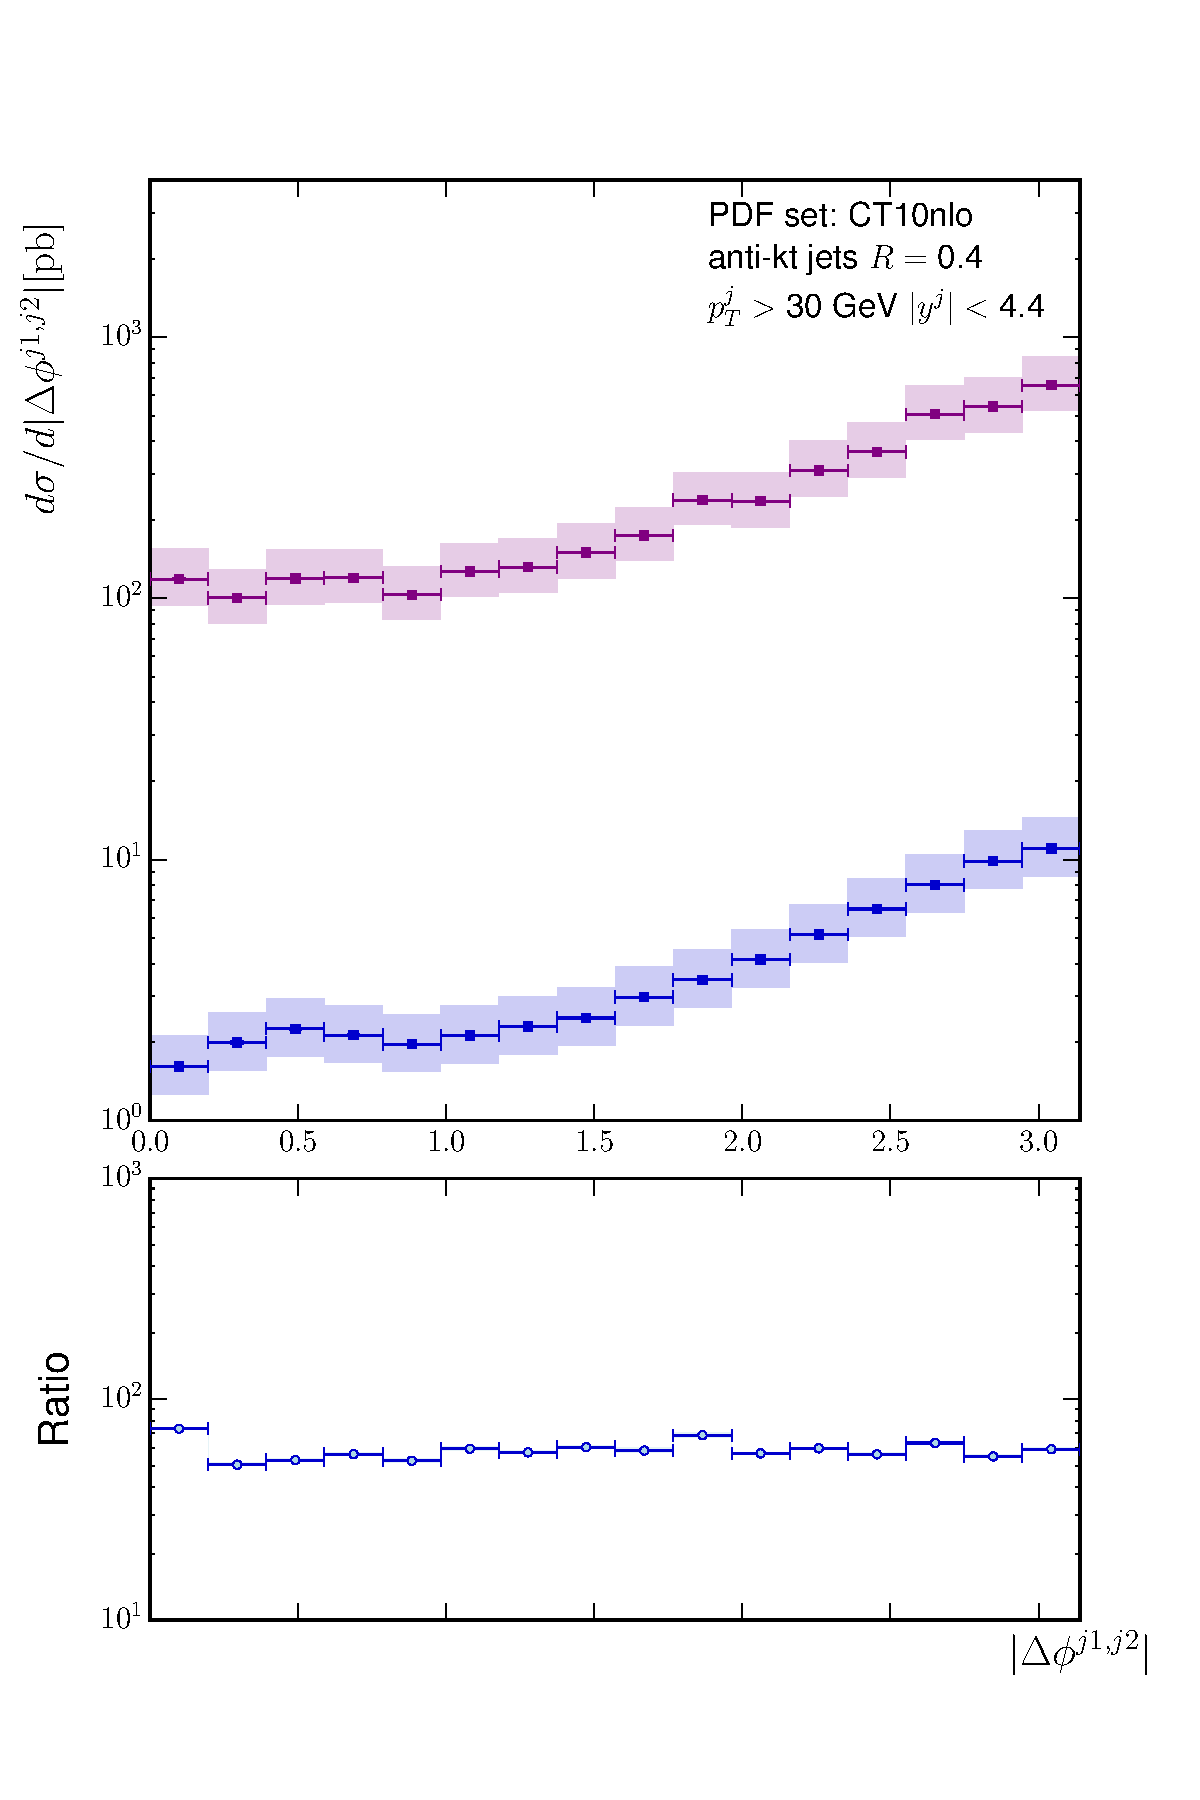
\includegraphics[width=0.8\linewidth]{ATLAS_Z_100TeV_12a}
		\caption{The differential cross-section for $\zg$ plus inclusive dijets as a function of the azimuthal seperation of the dijet system shown for
		         centre-of-mass energies of 7TeV (blue) and 100TeV (pink).}
		\label{fig:100tev_12a}
	\end{figure}

	Fig. (\ref{fig:100tev_12a}) notes:

	\begin{itemize}
		\item dphi plot
		\item Start with this one because its the most boring,
		\item i.e. if QCD didnt change with energy scale all plots would be like this one
	\end{itemize}

	\begin{figure}[h]
		\centering
		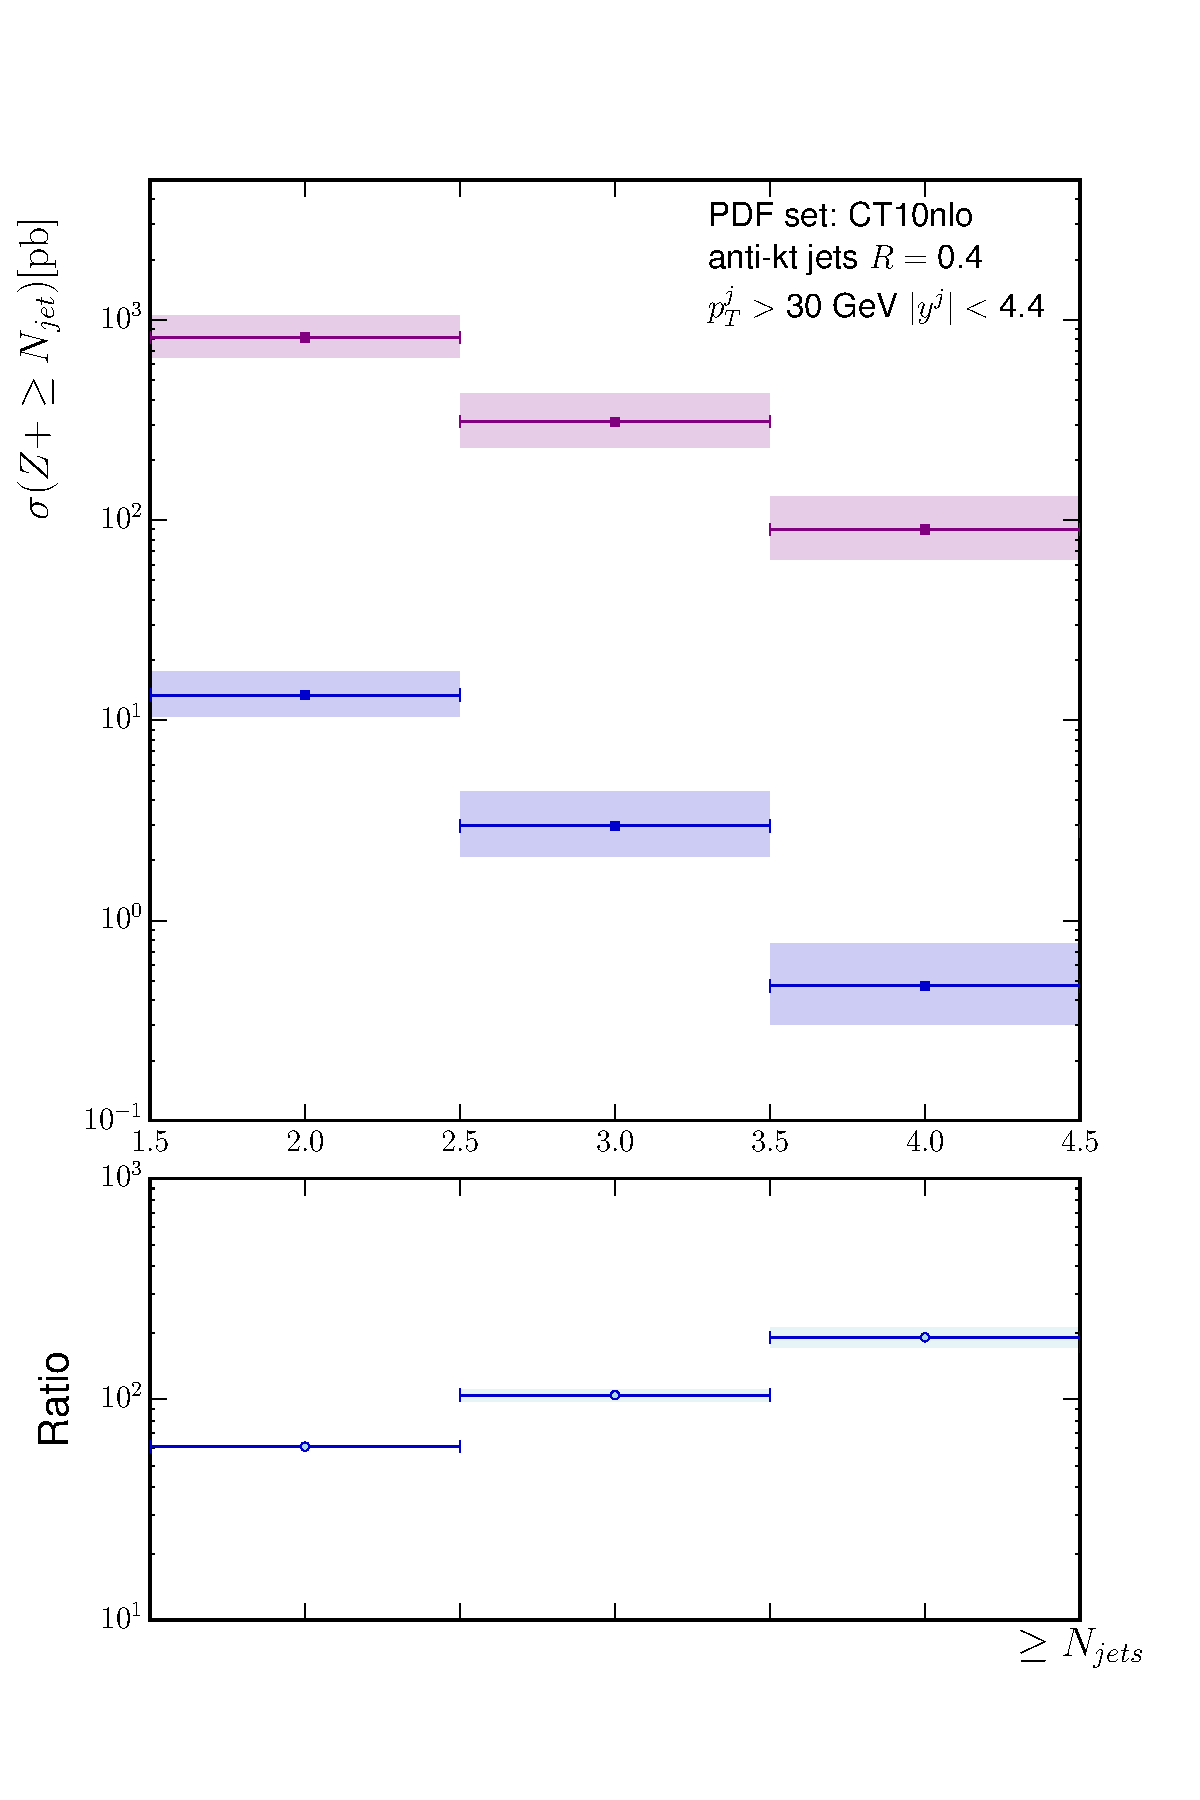
\includegraphics[width=0.8\linewidth]{ATLAS_Z_100TeV_2a}
		\caption{The cross-section for $\zg$ plus inclusive dijets as a function of the number of jets $N_{\text{jet}}$ shown for
		         centre-of-mass energies of 7TeV (blue) and 100TeV (pink).}
		\label{fig:100tev_2a}
	\end{figure}

	Fig. (\ref{fig:100tev_2a}) notes:

	\begin{itemize}
		\item njets,
		\item Explicitly shows that the break-down of the perturbative series gets worse at higher energies,
		\item The contributions from higher-order corrections increase as the energy increases,
	\end{itemize}

	\begin{figure}[h]
		\centering
		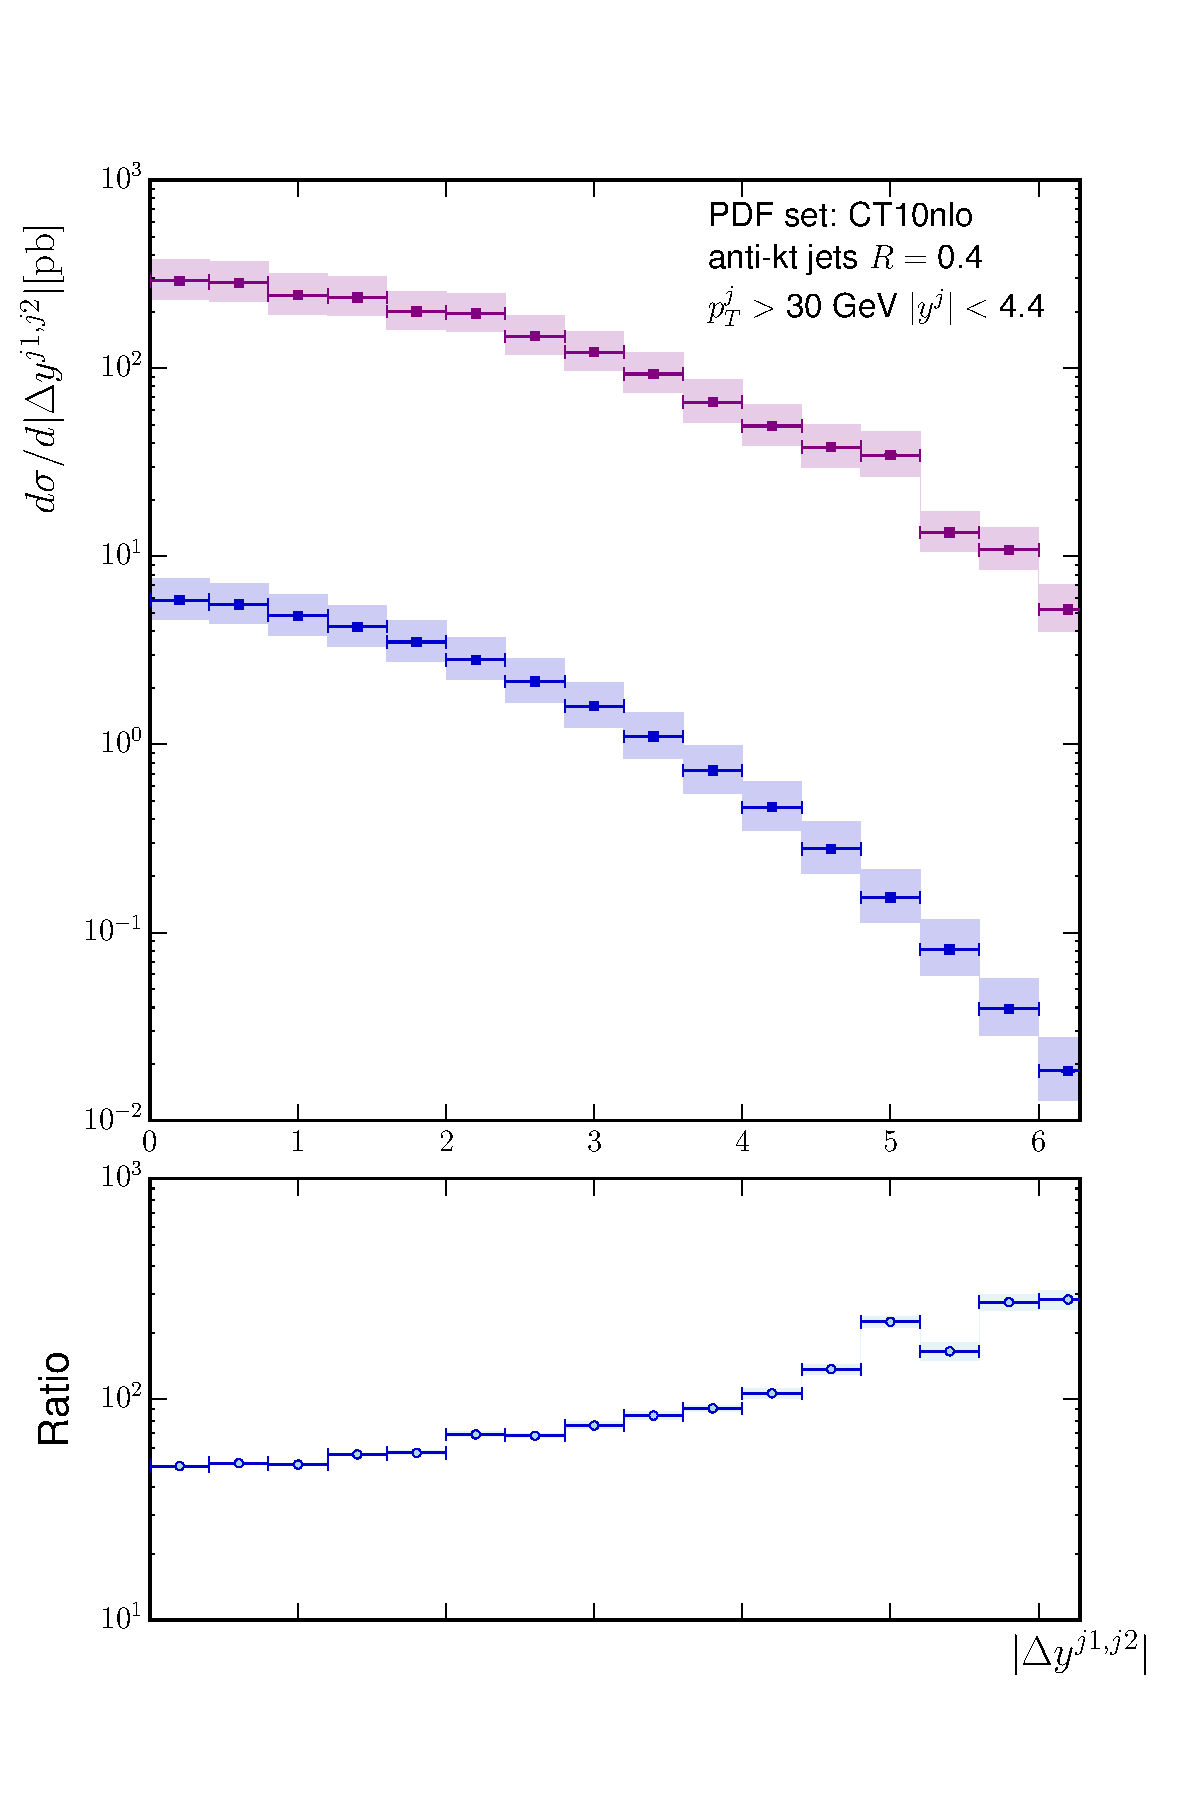
\includegraphics[width=0.8\linewidth]{ATLAS_Z_100TeV_11a}
		\caption{The differential cross-section for $\zg$ plus inclusive dijets as a function of the absolute value of the
		         rapidity gap between the dijets, $\Delta y^{j1, j2}$ shown for centre-of-mass energies of 7TeV (blue) and
		         100TeV (pink).}
		\label{fig:100tev_11a}
	\end{figure}

	Fig. (\ref{fig:100tev_11a}) notes:

	\begin{itemize}
		\item dy plot,
		\item O(10) increase in cross-section as we go to large rapidities,
		\item More energy in initial state means we can get more jets further in to the outer regions of y-space,
		\item The increase seen is \emph{exactly} the large logs we capture at play
	\end{itemize}

	\begin{figure}[h]
		\centering
		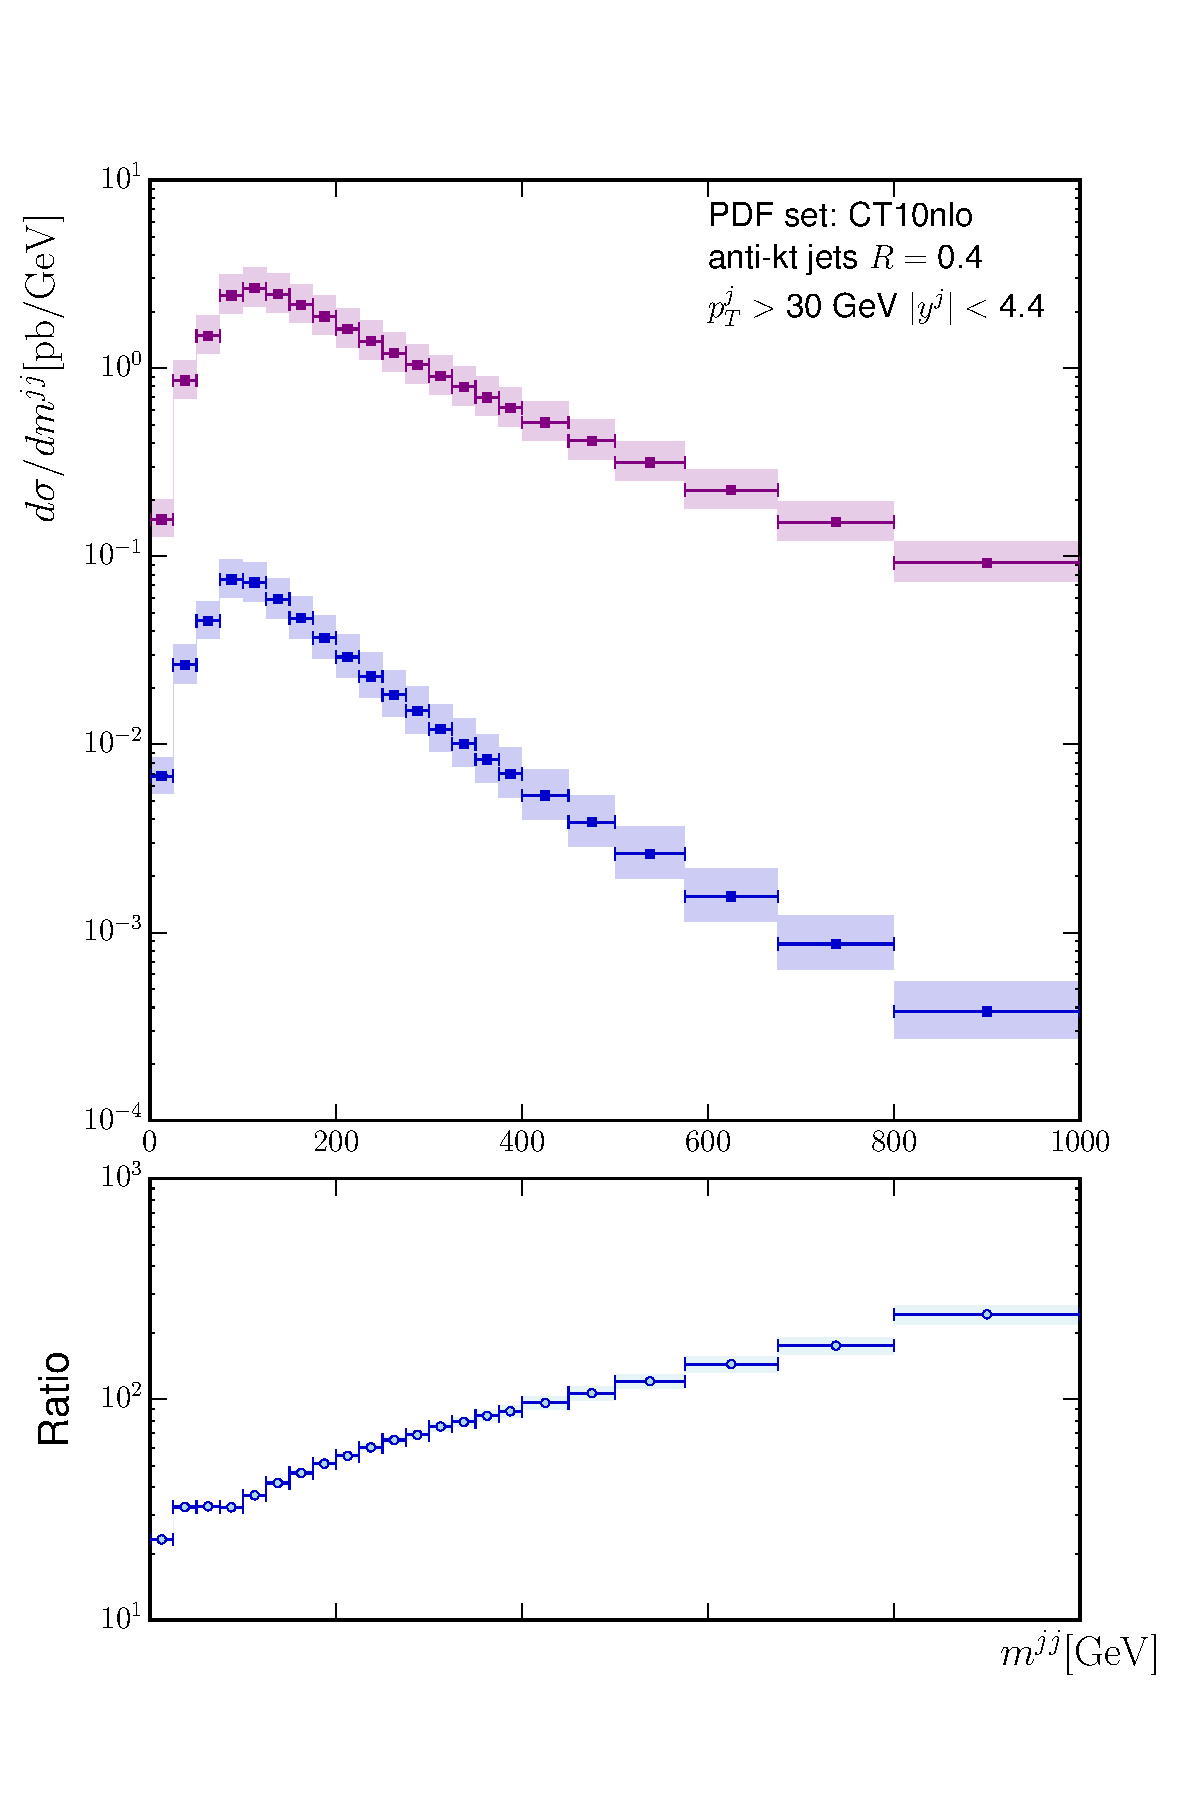
\includegraphics[width=0.8\linewidth]{ATLAS_Z_100TeV_11b}
		\caption{The differential cross-section for $\zg$ plus inclusive dijets as a function of the invariant mass
		         of the dijets, $m^{jj}$, shown for centre-of-mass energies of 7TeV (blue) and 100TeV (pink).}
		\label{fig:100tev_11b}
	\end{figure}

	Fig. (\ref{fig:100tev_11b}) notes:

	\begin{itemize}
		\item $dm_jj$ plot,
		\item O(10) increase in cross-section as we go to large invariant masses,
		\item Invariant masses again correlate with the logs we resum (show this explicitly if you havent already),
		\item Similar to fig. (\ref{fig:100tev_11a})
	\end{itemize}

	\begin{figure}[h]
		\centering
		\begin{subfigure}[b]{0.48\textwidth}
			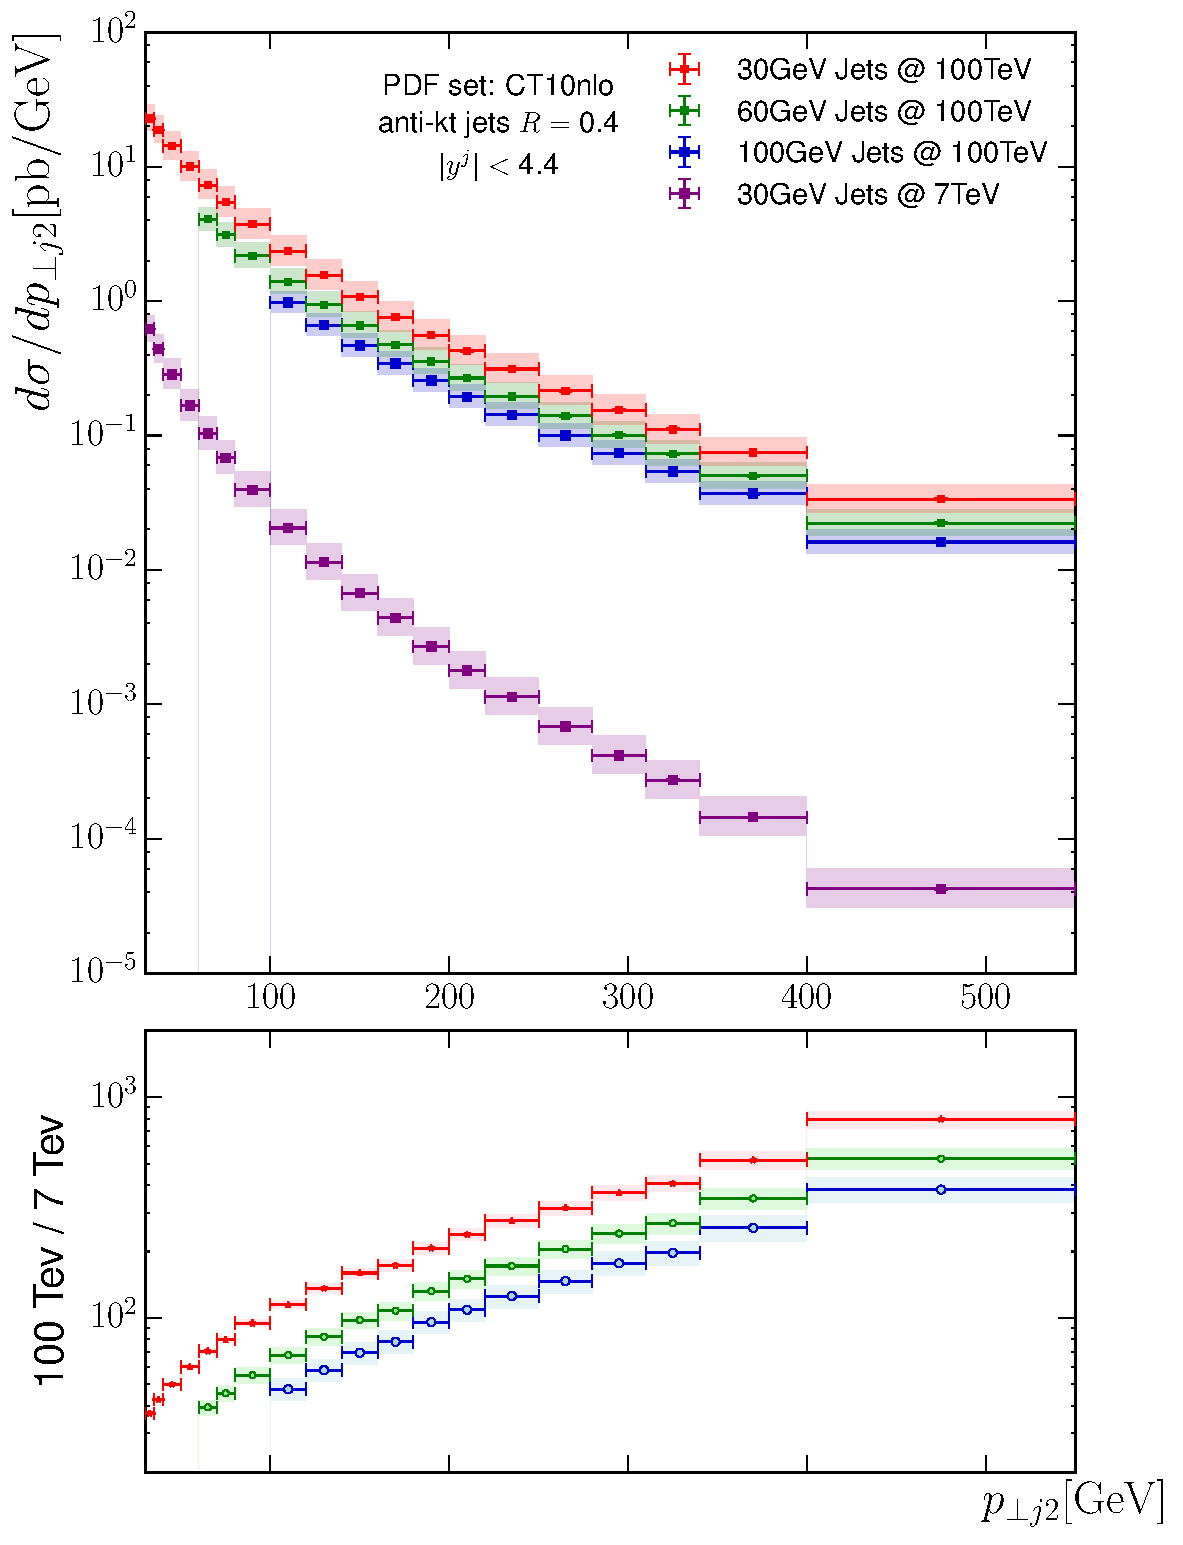
\includegraphics[width=\textwidth, height=1.3\textwidth]{ATLAS_Z_100TeV_5b}
			\caption{}
			\label{fig:100tev_5b}
		\end{subfigure}

		\begin{subfigure}[b]{0.48\textwidth}
			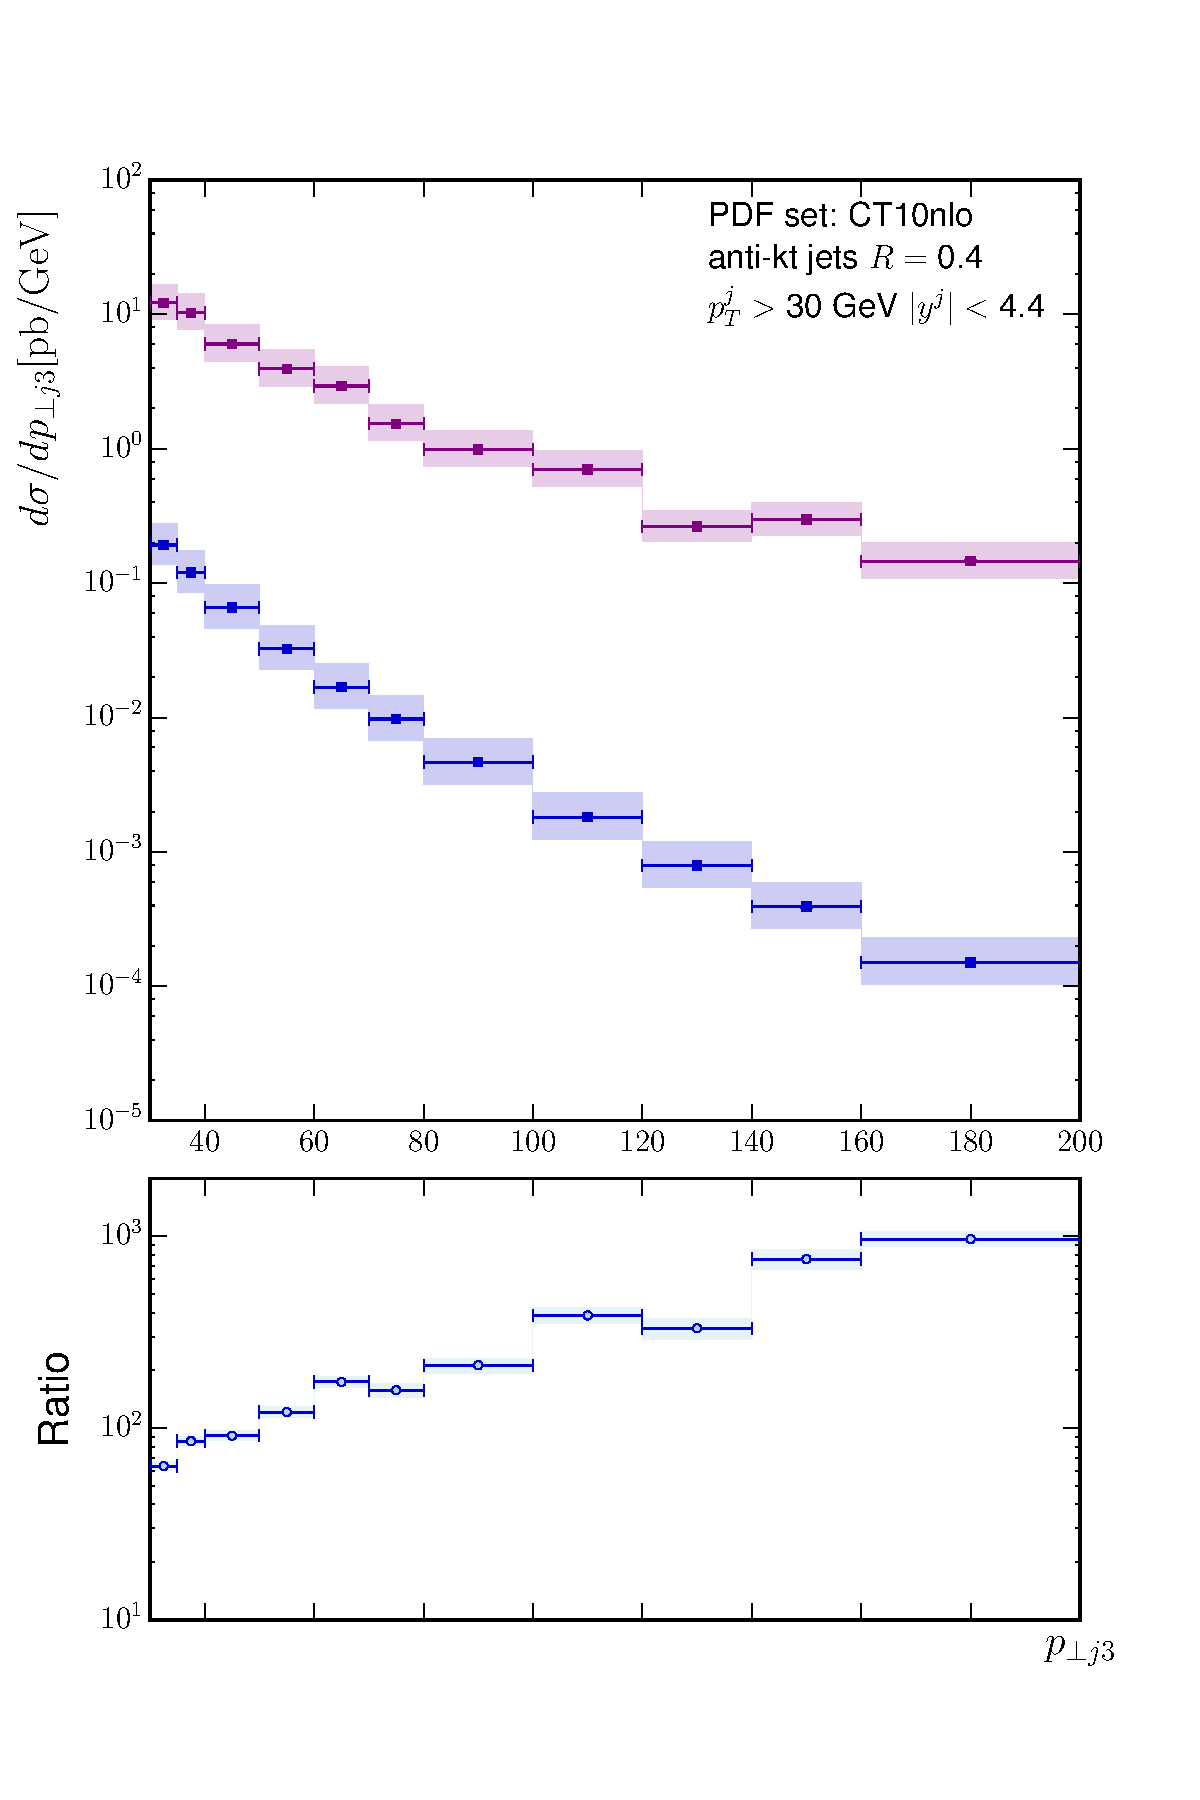
\includegraphics[width=\textwidth, height=1.3\textwidth]{ATLAS_Z_100TeV_6a}
			\caption{}
			\label{fig:100tev_6a}
		\end{subfigure}
		~
		\begin{subfigure}[b]{0.48\textwidth}
			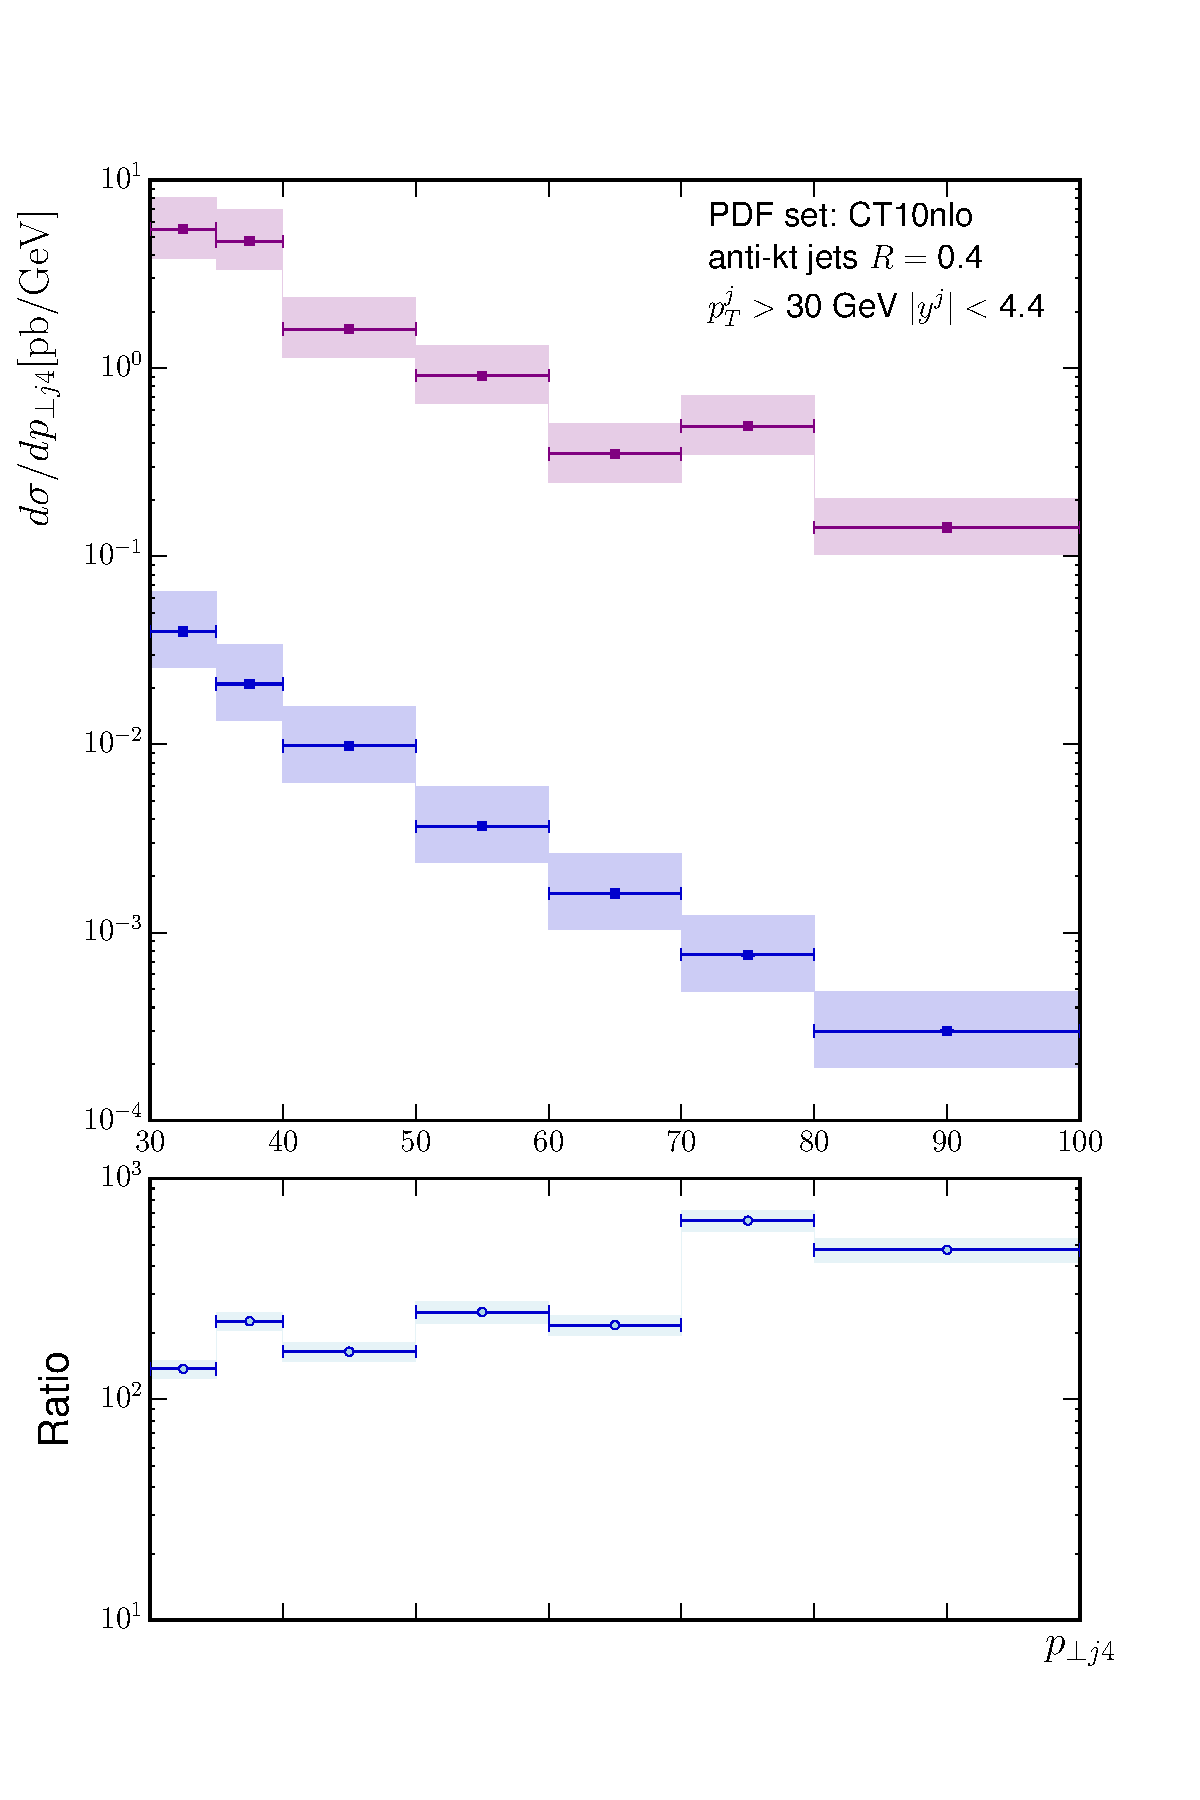
\includegraphics[width=\textwidth, height=1.3\textwidth]{ATLAS_Z_100TeV_6b}
			\caption{}
			\label{fig:100tev_6b}
		\end{subfigure}
		\caption{The differential cross-section for $\zg$ plus inclusive dijets as a function of the transverse momentum
		         of the first, second and third leading jets in $p_T$ shown in fig. \ref{fig:100tev_5b}, \ref{fig:100tev_6a}
		         and \ref{fig:100tev_6b} respectively and for centre-of-mass energies of 7TeV (blue) and 100TeV (pink).}
	\end{figure}

	Fig. (\ref{fig:100tev_5b}-\ref{fig:100tev_6b}) notes:

	\begin{itemize}
		\item pT distributions,
		\item Heavy tails...soooo?
		\item More energy in initial state means we can get more jets further in to the outer regions of y-space,
		\item What effect would a shower have on these distributions?  Plenty of spare pT to radiate.
	\end{itemize}

	\begin{figure}[h]
		\centering
		\begin{subfigure}[b]{0.48\textwidth}
			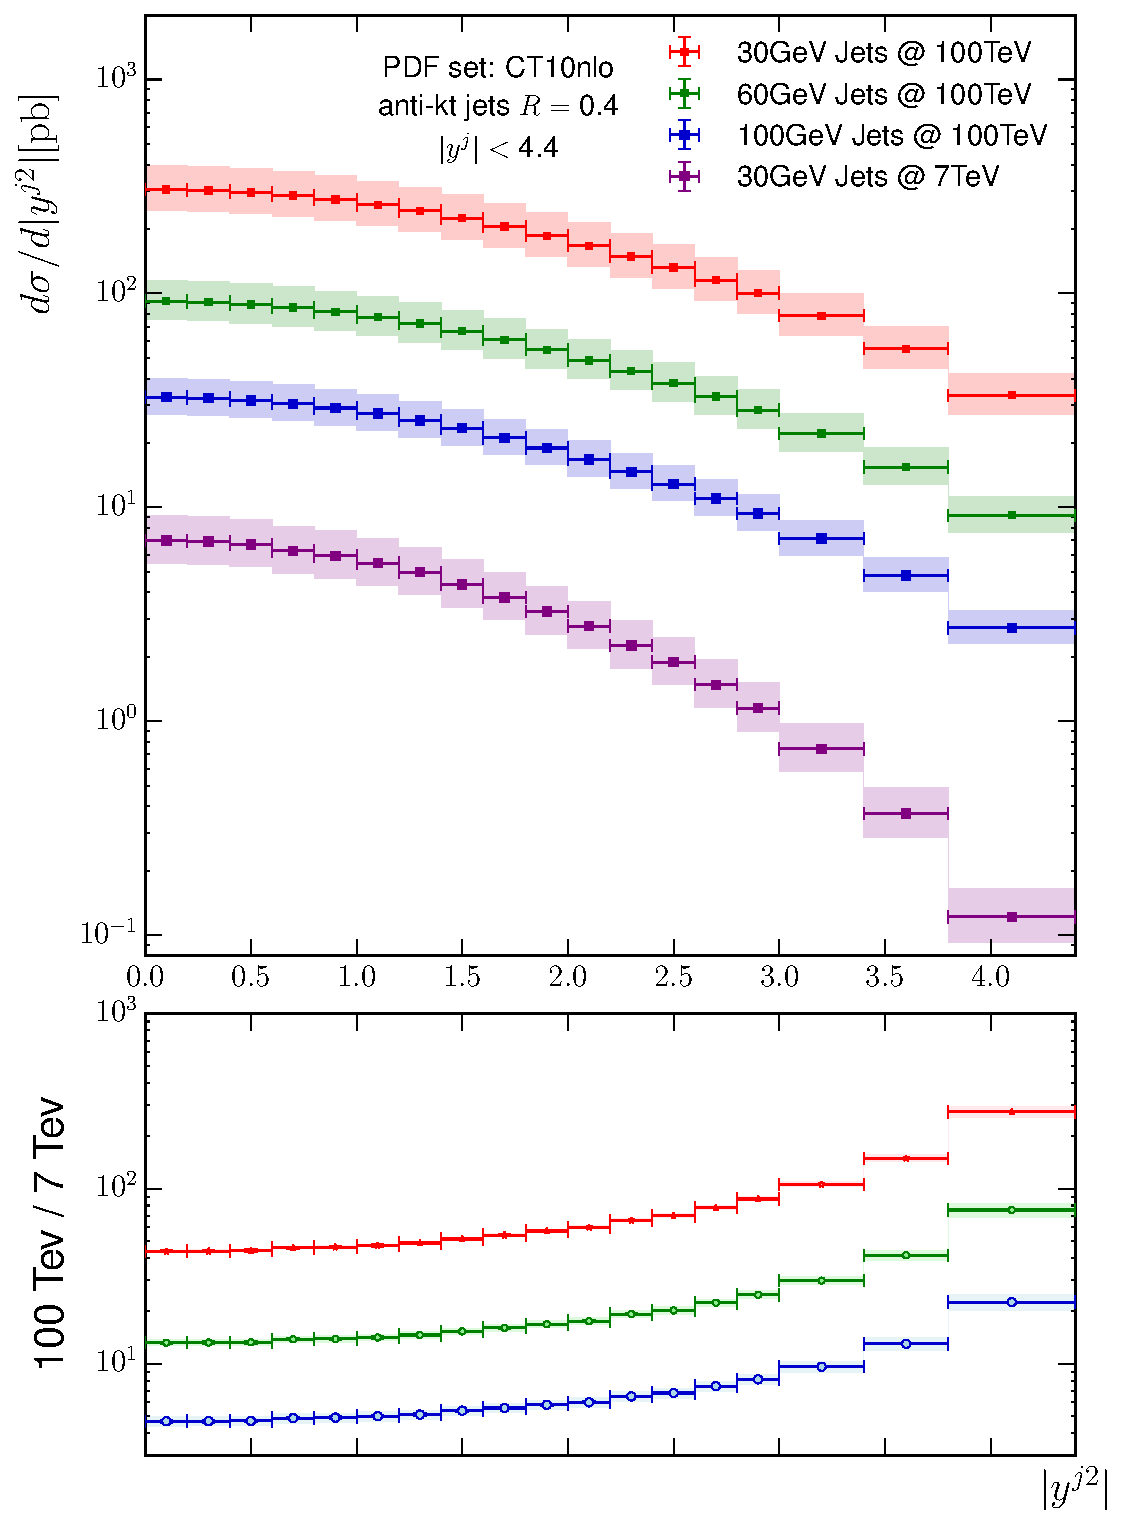
\includegraphics[width=\textwidth, height=1.3\textwidth]{ATLAS_Z_100TeV_9b}
			\caption{}
			\label{fig:100tev_9b}
		\end{subfigure}

		\begin{subfigure}[b]{0.48\textwidth}
			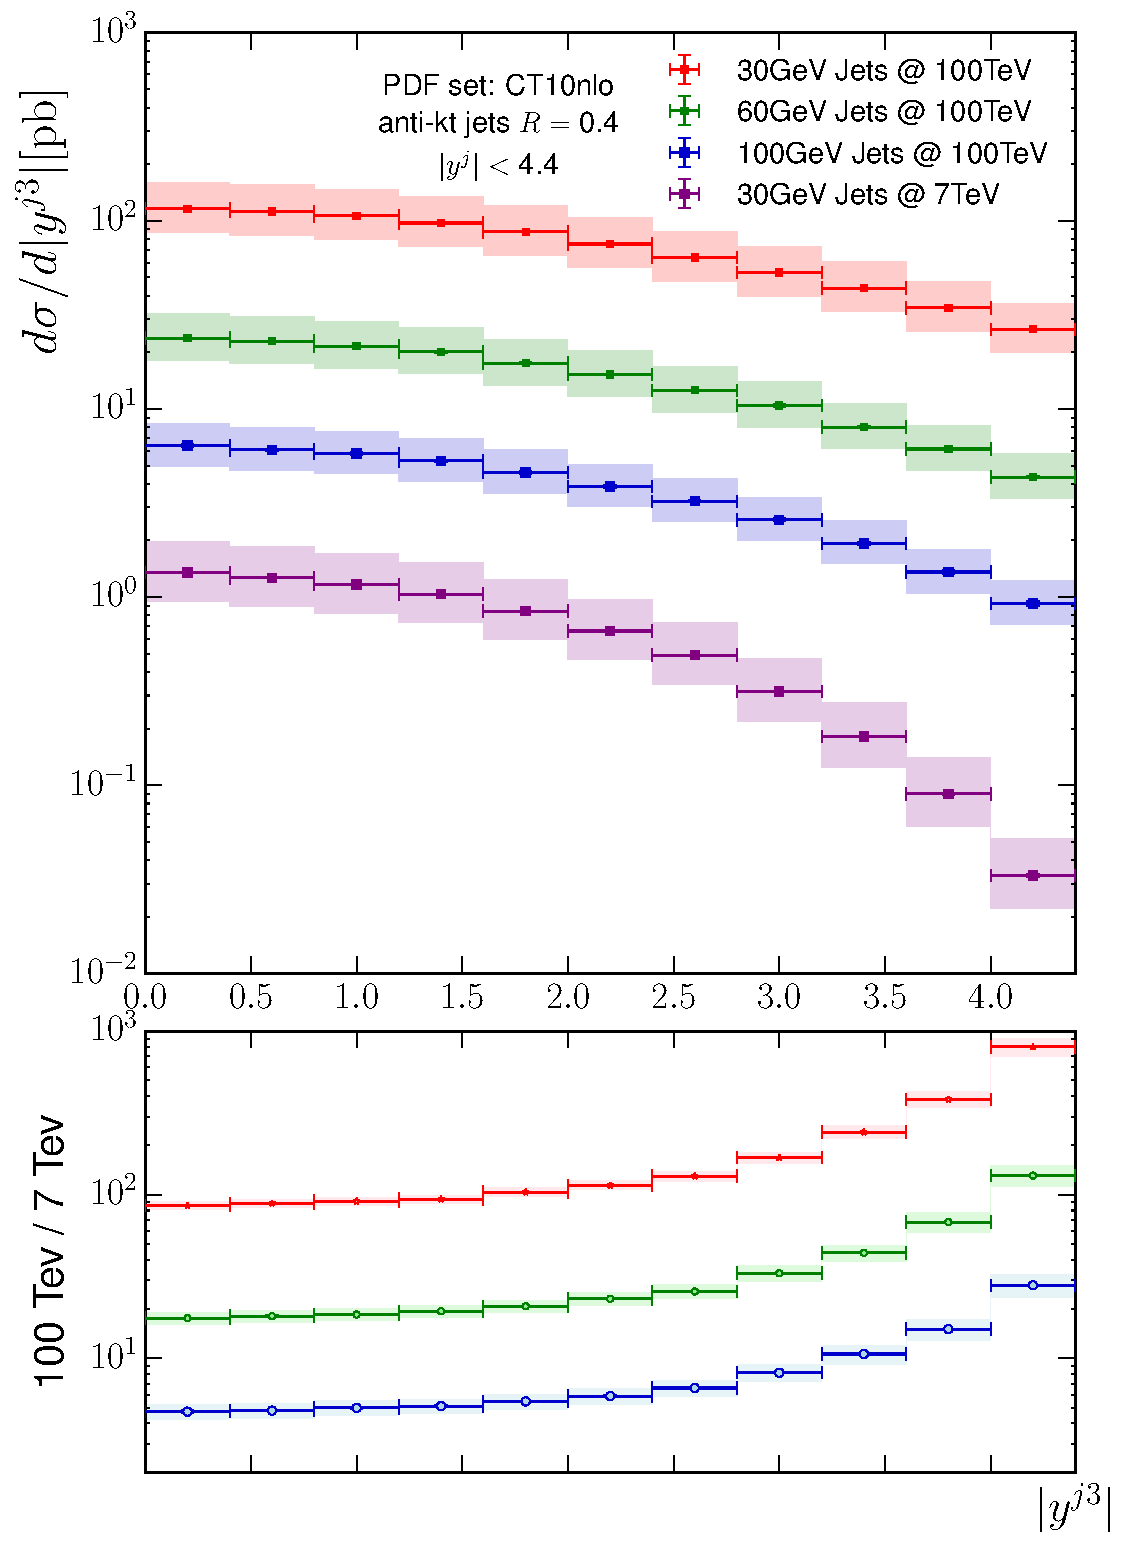
\includegraphics[width=\textwidth, height=1.3\textwidth]{ATLAS_Z_100TeV_10a}
			\caption{}
			\label{fig:100tev_10a}
		\end{subfigure}
		~
		\begin{subfigure}[b]{0.48\textwidth}
			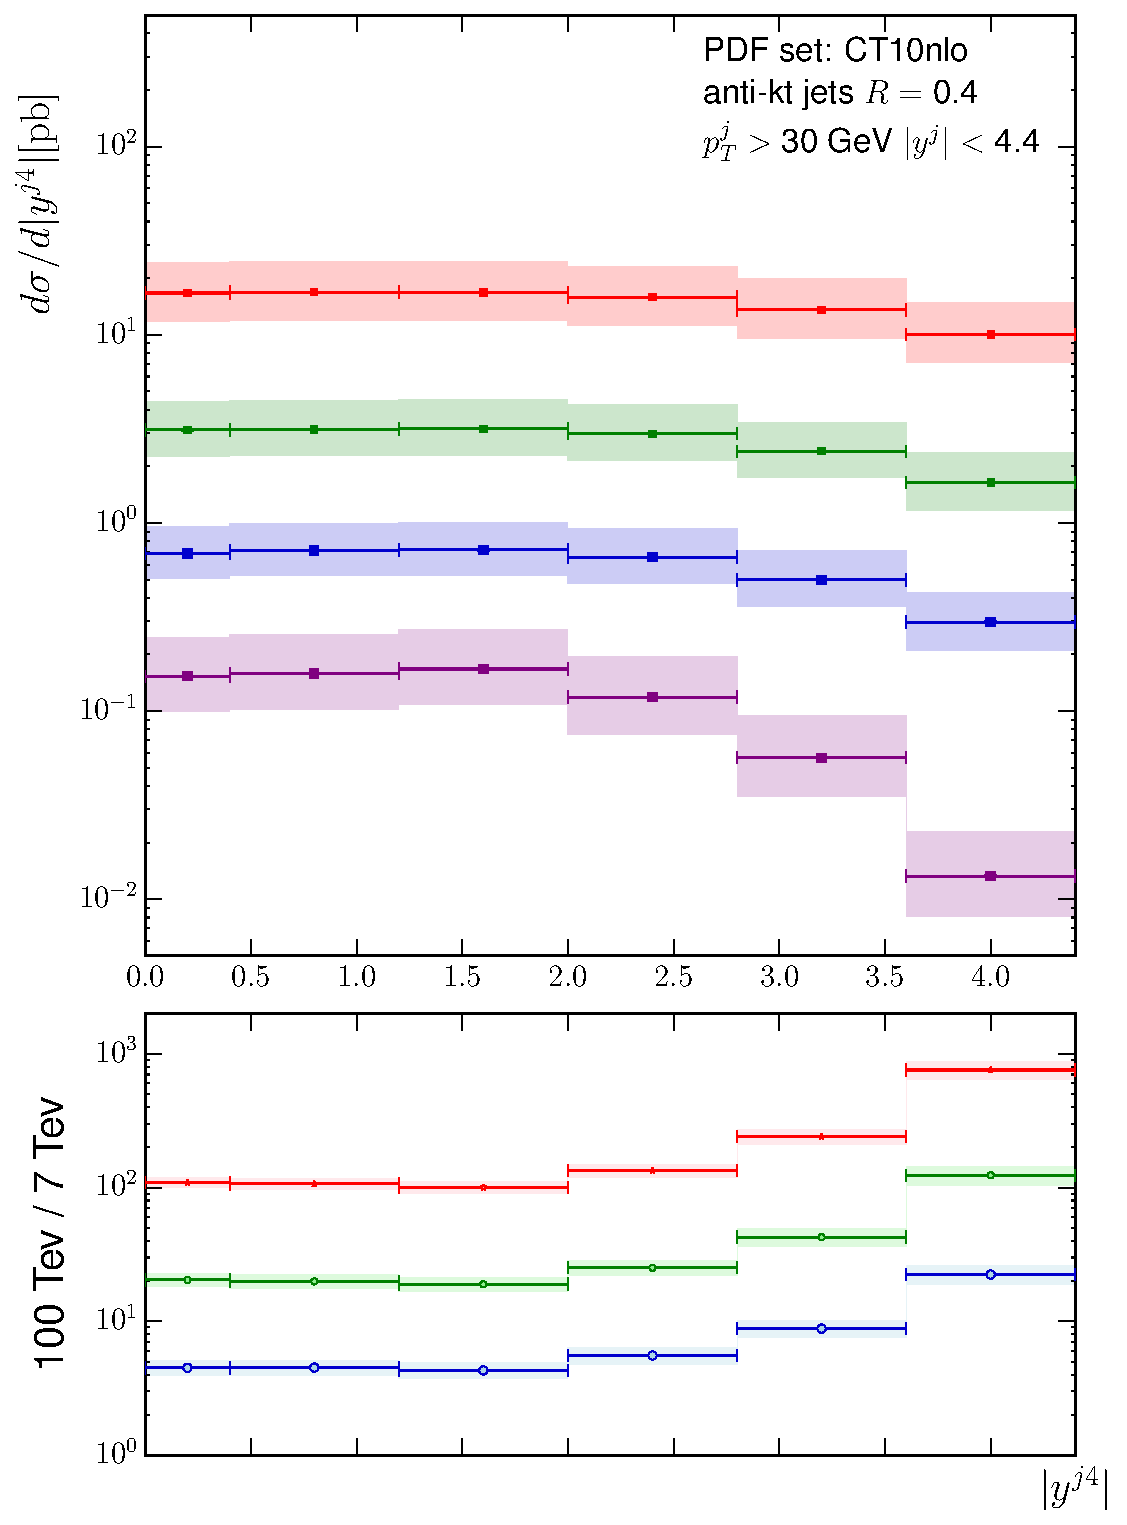
\includegraphics[width=\textwidth, height=1.3\textwidth]{ATLAS_Z_100TeV_10b}
			\caption{}
			\label{fig:100tev_10b}
		\end{subfigure}
		\caption{The differential cross-section for $\zg$ plus inclusive dijets as a function of the absolute value of the rapidity
		         of the first, second and third leading jets in rapidity shown in fig. \ref{fig:100tev_9b}, \ref{fig:100tev_10a}
		         and \ref{fig:100tev_10b} respectively and for centre-of-mass energies of 7TeV (blue) and 100TeV (pink).}
	\end{figure}

	Fig. (\ref{fig:100tev_9b}-\ref{fig:100tev_10b}) notes:

	\begin{itemize}
		\item Not much more to say about these - mostly covered in dy plots,
	\end{itemize}

